\documentclass[12pt,preprint]{aastex}
\usepackage{url}
\usepackage{natbib}
\usepackage{graphicx}
\usepackage{subfig}
\usepackage{algorithmic}
\usepackage{appendix}
\usepackage{gensymb}
\usepackage{amsmath}
%\usepackage{fixltx2e}



%%%%%%%%%%%%%%%%%%%%%%%%%%%%%%%%%%%%%%%%%%%%%%%%%%%%
%%% author-defined commands
\newcommand\x         {\hbox{$\times$}}
\def\mic              {\hbox{$\mu{\rm m}$}}
\def\about            {\hbox{$\sim$}}
\def\Mo               {\hbox{$M_{\odot}$}}
\def\Lo               {\hbox{$L_{\odot}$}}

%\captionsetup[figure]{labelformat=simple}
%%%%%%%%%%%%%%%%%%%%%%%%%%%%%%%%%%%%%%%%%%%%%%%%%%%%

% Abstract




\begin{document}

\title{Moving Object Pipeline System Design}

\author{Jonathan Myers, Lynne Jones, Tim Axelrod}

\begin{abstract}

The Moving Object Pipeline System (MOPS) has two responsibilities
within LSST Data Management.  First, it is responsible for generating
and managing the \textbf{Moving Object} data products.  The Moving
Objects are identified solar system objects (SSOs) with associated
Keplerian orbits, errors, and detected sources associated with those
solar system objects.  The second responsibility of the MOPS is to
predict future locations of moving objects in incoming images so that
their sources may be associated with known objects; this will reduce
the number of transient detections and prevent Alert Generation on
detections of known Solar System objects.  Design for the MOPS
component is based closely on the design of the PanSTARRS MOPS.

\end{abstract}

\tableofcontents


\section{System Design and Responsibilities}

The Moving Object Pipeline System has two main responsibilities: the
generation and maintenance of the Moving Object database, and the
prediction of known object locations which are sent to the Association
Pipeline to prevent unneccessary alerts.  The MOPS has been broken
into two components, colloquially known as ``DayMOPS'' and ``NightMOPS.''
 

\begin{figure}[!ht]
\centering
  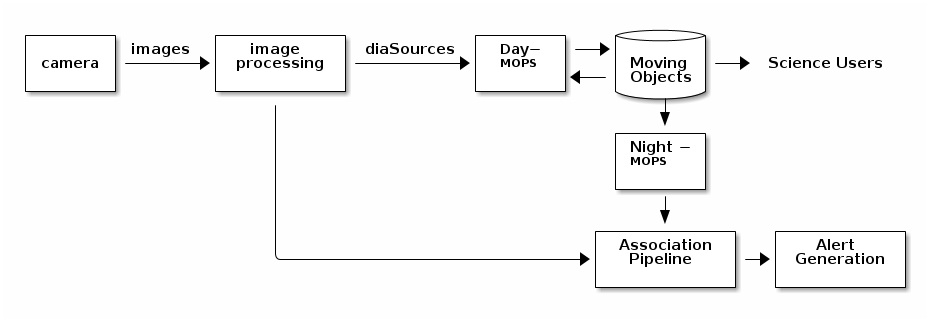
\includegraphics[width=13cm]{illustrations/mopsWithinLsst.png}
\caption{ Data flow from the camera through DayMOPS to the Science
  Users and Alert Generation.  DayMOPS will build and maintain the
  Moving Objects table, NightMOPS will use the Moving Objects table to
  communicate with the Assocation Pipeline.  }
\label{mopsWithinLsst}
\end{figure}


``DayMOPS,'' so called because it processes data acquired from the
previous night in a large batch operation, is responsible for
discovering new Moving Objects in newly-acquired data, searching old
data for detections of new objects, and updating the Moving Objects
table to reflect newly-acquired data. It is also responsible for
periodically cleaning and refining the contents of the Moving Objects
table.  ``NightMOPS'' is responsible for projecting the locations of known
Moving Objects in upcoming images as they are announced during
night-time operations.  

The relationship between DayMOPS, NightMOPS and the neighboring
components of the LSST Data Management system is illustrated in
figure \ref{mopsWithinLsst}.

\subsection{DayMOPS: Discovering and Managing Moving Objects}

% Illustration of DayMOPS

% sky-plane vs. orbit-space illustration

The DayMOPS is responsible for discovering moving objects in source
catalogs.  The task of discovering and tracking asteroids has been
performed by humans since hundreds of years ago, but automated systems
for asteroid discovery and tracking remain relatively uncommon.  Other
surveys have often mixed human and computerized approaches -
\textbf{can we get some more history here?}.


The design of the LSST DayMOPS is based on the PanSTARRS Moving Object
Pipeline System \citep{psMOPSDesign}.  The approach used here is to
first find sets of detections with sky-plane paths consistent with
asteroid behaviour; these sets of detections and their fitted paths
are called \textbf{tracks}.  A set of algorithms for the discovery of
sky-plane tracks in dense data are presented in
\citet{Kubica:2005:MTA:1081870.1081889}; these algorithms are the
basis of the linking methods for the current LSST DayMOPS.


%% TBD: it would be really nice to have some illustrations here
%% showing detections of an object, and possibly tracklets and tracks
%% as well

The tracking methods used are based on a tiered approach; first two or
more detections from a single night are linked into
\textbf{tracklets}, which represent a hypothetical object and a linear
approximation of its sky-plane motion.  These tracklets are later
joined into larger tracks. Because of the increasing complexity of
sky-plane motion over time, we are generally interested in tracks
which span no more than 15-30 days of observation time.

The PanSTARRS MOPS uses a fairly loose and generous approximation of
asteroid motion.  This allows for many mislinkages or \textbf{false
  tracks}, combining detections which are not attributable to the same
source, but virtually all objects for which a true (correctly-linked)
track could be generated will get some correct track.  With LSST's
expected density of detections, we found that this glut of false
tracks was generally too painful.  As a result, our methods diverge
from those of PanSTARRS as we introduce some more strict filters on
tracks, reducing the number of mislinkages at the expense of
potentially missing some true tracks.  The algorithms, their
implementations, the additional filters, and their behaviors are
presented thoroughly in Chapter \ref{linking}.

Once tracks are discovered, they are sent to the Orbit Determination
phase. The Orbit Determination phase takes these sets of sky-plane
detections and attempts to find a Keplerian orbit which could generate
the detections.  This orbit is further refined, and error bounds are
established, using differential correction.  Orbit Determination will
reject many tracks as false, but should successfully find precise
orbits for virtually all correctly linked tracks.  Several methods for
performing this task are known, and several have open-source implementations
available to LSST \citep{Milani04orbitdetermination},
\citep{Milani2006}, \citep{OpenOrb2009}, \citep{granvik_thesis}.  The
orbits discovered by Orbit Determination, and the detections present
in the track associated with each orbit, are used to generate new
Moving Objects.

\begin{figure}[h]
\begin{center}
  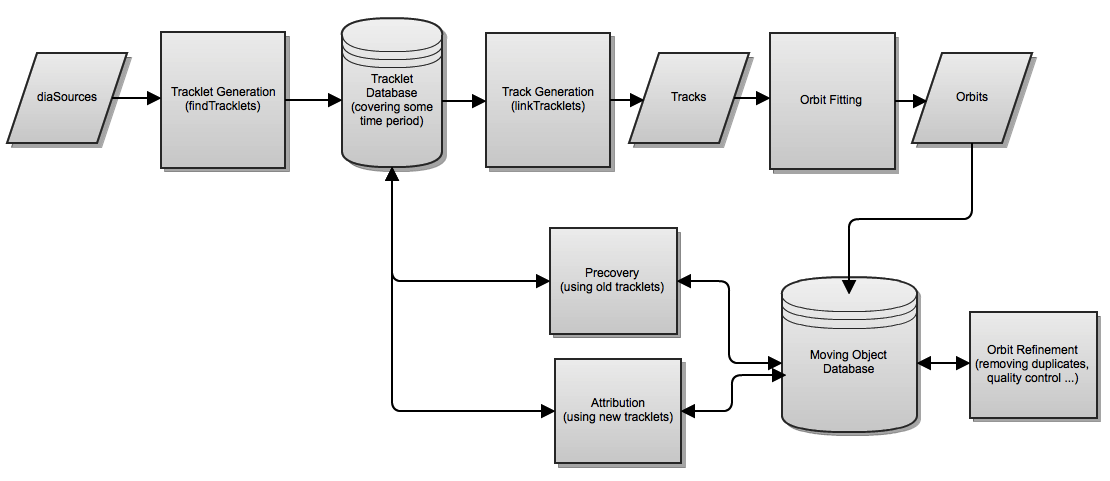
\includegraphics[width=11cm]{illustrations/mopsDiagram.png}
\end{center}
\caption{ Data flows into the DayMOPS pipeline and results in
  modifications of the Moving Objects table in a variety of ways,
  including attribution to known objects, a multi-stage pipeline for
  the discovery of new objects, and periodic refinements of the Moving
  Object table, such as possible merges of redundant objects or
  removal of false orbits. }
\label{mopsDiagram}
\end{figure}



The DayMOPS is expected to perform several additional tasks to manage
and improve the Moving Objects table over time.  Attribution is the
process of identifying known objects in incoming data and adding those
detections to the correct Moving Object, in a process called
Attribution. Similarly, Precovery is the recovery of known,
unattributed detections associated with a newly-discovered Moving
Object.  Another refinement is the merging of potentially redundant
Moving Objects.  The complete set of DayMOPS tasks and their data
flows are illustrated in figure \ref{mopsDiagram}.






\section{DayMOPS}
\label{linking}

Sufficiently bright moving objects which are observed by the LSST
telescope will generate DiaSource detections, stored in the LSST
DiaSource detection catalog.  The LSST DiaSource detection catalog
will also hold detections from a variety of non-moving object sources,
including transient phenomena and artifacts of image processing.

The LSST DayMOPS system is responsible for finding previously unknown
moving objects within the LSST DiaSource catalog.  Due to the large
number of detections expected, and the sometimes-unpredictable
behavior of asteroids with unknown orbits, a structured and
carefully-designed system is necessary to perform this searching and
discovery in a computationally efficient manner.






\subsection{Orbits}
Heliocentric orbits describe an orbit around the Sun.  Generally,
asteroids, planets and other solar system objects follow elliptical
paths, with the Sun as their focal point.  These paths are described (in general
practice as well as the LSST Moving Objects catalog) with a Kepler
orbit, which describes an ellipse using six parameters. 

For purposes of DayMOPS and NightMOPS, we assume that a well-fitted
Kepler orbit should be sufficient to predict the location of an object
well into the future or past.  

To simplify the problem, we will not attempt to deal with objects
which do not follow conventional heliocentric orbits, such as
loosely-coupled binaries or planetary satellites.


\textbf{TBD: Illustration of a Kepler orbit - Wikipedia has a good one.}


\subsection{Orbit Determination and The Linking Problem}
Orbit determination refers to the problem of identifying an object's
orbit given a well-spaced set of detections of that object.  The
problem of orbit determination has been studied extensively \textbf{
  CITATIONS HERE }, and several software tools exist which can, given
a set of detections, identify an orbit which could have generated them
or identify that no such orbit could exist.We entrust that a suitable
outside tool will be chosen to handle this problem.

This leads to the non-trivial problem of correctly grouping sets of
detections by the unknown object which generated them, and reporting
these detections to an orbit determination tool.  This is the \textbf{
  linking problem}.  The majority of efforts in the DayMOPS system
have been directed at constraining the number of linkages which are
passed to the orbit determination tool, and at methods for discovering
those linkages quickly.

Fortunately, the well-known linear and quadratic approximations of asteroid
motion can be used both to predict possible linkages, and reject those
which are obviously untenable.  

\subsubsection{Linear and Quadratic Models}

\begin{figure}[ht]
  \centering
    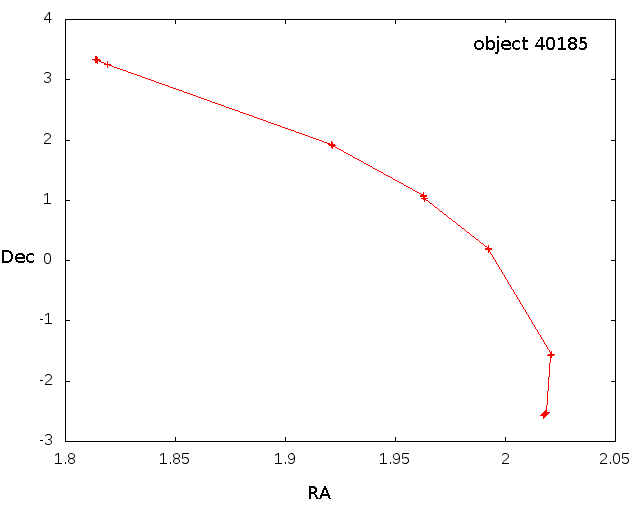
\includegraphics[width=10cm]{illustrations/4.png}
    \caption{ A plot of simulated observations of object 40185 on the
      sky.  Though the observations span only one week, a pronounced
      quadratic path is visible.  Note that the object is observed two
      or more times on each night.}
\label{objectPlotted}
\end{figure}



In order to discover and identify new objects, astronomers have
traditionally used sky-plane approximations to predict and model the
behavior of solar system objects for which a true orbit is not yet
known.  As a general rule of thumb, objects are said to move linearly
(with a more or less fixed velocity) in RA and Dec over the course of
a single night and quadratically (having velocity and some
acceleration) in RA and Dec over the course of a month.  These are, of
course, approximations, and linear and quadratic fits will inevitably
contain some error.  An example of one object with a clear quadratic
path over seven days is show in Figure~\ref{objectPlotted}.

Given many detections which may or may not be attributable to one or
more asteroids, these approximations are used to help determine which
detections could plausibly be linked.  If several detections over the
course of a single night do not follow a roughly linear path, we trust
that they could not have been attributable to the same object; if
several detections over the course of a month do not follow a roughly
quadratic path, we will trust that they could not be attributable to
the same object.  By ignoring the obviously implausible linkages, we
significantly reduce the number of hypothetical linkages we must
investigate.

Of course, since these are merely approximations, it is almost
inevitable that some correct linkages will be rejected.  In
particular, some near-Earth-objects (NEOs) may exhibit sky-plane
behaviour not consistent with these rules of thumb.


\subsubsection{Higher-order Sky-Plane Models}
\textbf{TBD: Tim's methods go here - the assumed topocentric distance, topocentric correction, higher-order fits}


\subsection{The Linking Pipeline}
The linking pipeline is responsible for finding sets of detections
which may be attributable to the same moving object and sending them
to the Orbit Determination stage, which will either accept them as a
true linkage with an associated orbit or reject them as incorrectly
linked.  

To deal with the scale and complexity of discovering plausible
multi-night linkages for unknown objects, the DayMOPS system is
designed as a pipeline of several stages, building increasingly
sophisticated linkages at each step until multi-night linkages
suitable for orbit determination are discovered.  Specifically, we
move from individual detections to nightly, linear \textbf{tracklets},
to eventual multi-night, quadratic \textbf{tracks} suitable for orbit
determination.  These tracks are filtered using a slightly more
sophisticated (but simpler than full orbit-space) model of asteroid
motion, to more quickly reject the (often numerous) mislinked tracks.


\textbf{TBD: Add an illustration of the various stages and a short piece of
introductory text.  Also perhaps useful: show one object's detections and its various states of linkage. (detections, tracklets, merged tracklets, track(s))}


Note that tracklets and tracks represent hypothetical linkages, many
of which may be incorrect.  A single detection may exist in several
tracklets and/or several tracks.  A given tracklet may be found in
multiple tracks.  Some detections may never be linked into any
tracklet; some tracklets will never be linked into any track.  

%The
%DayMOPS system is built using methods and algorithms intended to
%efficiently find plausible hypothetical linkages without wasting much
%computational time or storage on finding unlikely linkages.


%% TBD: Describing topocentric correction goes here?  It has to go
%% somewhere.  It is only performed on the data sent to linkTracklets,
%% but this isn't really central to understanding the vtrees algorithm
%% - though it does effect the data ``seen'' by linkTracklets
%% throughout.


\subsection{Building Tracklets}

\textbf{ possible illustration: show Dec/time for two images, then tracklets in Dec/time}

\textbf{Tracklets} are linkages between DiaSource detections occuring
within the same night. By creating tracklets, DayMOPS can find
sky-plane position and velocity estimates for sets of detections which
may belong to the same solar system objects.  The use of tracklets
also simplifies the downstream work of track generation, which
attempts to find sets of detections with a good
position/velocity/acceleration fit on the sky-plane; since tracklets
have known position and velocity, the track generation phase needs
only to find those tracklets compatible within some acceleration
factor.

Correctly-linked tracklets from a given object are needed to generate
a good track for that object and eventually discover its orbit.
However, if these useful tracklets are too deeply buried among very
large numbers of other tracklets, then the job of tracklet linking
will become extremely slow and expensive.  Generally, these other,
unwanted tracklets are false tracklets (mislinkages between detections
not attributable to the same object), though in special conditions
large numbers of correctly-linked but redundant tracklets can cause
pain as well (this will discussed in \ref{collapseTracklets}).

In order to ensure that tracklet-generating images are acquired, it is
necessary to ensure that fields of the sky are visited two or more
times within an accepted time period each night. To constrain the
number of tracklets, we impose a maximum apparent velocity on the
tracklets, and also require that sky fields be revisited within a
fairly short time period ($\leq 90$ minutes is the current rule).
Raising the maximum velocity threshold enables one to find
faster-moving objects, and raising the maximum allowed revisit time
also enables one to generate tracklets in more fields of the sky;
however, increasing either of these thresholds also increases the
search space and can significantly increase the number of mislinked
tracklets, greatly increasing the cost downstream.




\subsubsection{The findTracklets Software}

The process of initial tracklet creation is accomplished by the
findTracklets software.  Later refinement of tracklets is accomplished
by collapseTracklets and additional filters.

\subsubsubsection{Algorithm} 

The findTracklets software is responsible for finding pairs of
detections which occur within a fixed time threshold, and have
apparent velocity below a given threshold.  For a given detection and
a set of image times, one can calculate the maximum distance an object
could have travelled at each time using the velocity limit.  To find
detections with which the query detection could be linked, one can
imagine searching a circular region in the later images based on this
distance.

\begin{figure}[ht]
  \centering
    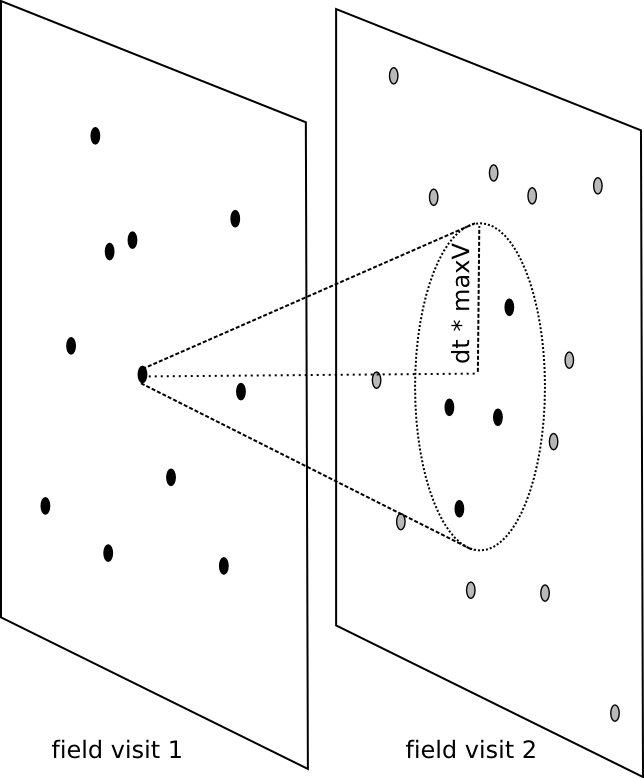
\includegraphics[width=6cm]{illustrations/findTracklets-onequery.png}
    \caption{ An example of searching for compatible second endpoints
      for a given detection.  The first detection and each of the
      second endpoints will be used to create a new tracklet.}
\label{findTrackletsIllustrated}
\end{figure}


Fortunately, this can be
accomplished in a fairly straightforward way through the use of
KD-Trees.  KD-Trees are a data structure which allows for quickly and
efficiently performing range searches on points in space
\citep{bentley_kdtrees}.  A KD-Tree-based method for building
tracklets was first contributed by Jeremy Kubica for his PhD thesis
\citep{kubica_thesis}.  For findTracklets, 2-Dimensional KD-Trees are
used, covering the space of (RA, Dec).  Given a detection and trees
containing detections from later images, we can use range searches to
quickly find nearby detections in those later images and use them for
the creation of tracklets.

\begin{figure}[ht]
\begin{algorithmic}
\REQUIRE $I$ is a set of images, each of which has an associated exposure time and contains a set of detections
\STATE \COMMENT{Create a 2D KD-Tree for each image, holding detections from that image.}
\STATE $T \gets \emptyset$
\FOR {$i \in I$}
  \STATE $t \gets$ Make2DTree$(i.detections)$
  \STATE $t.time \gets i.time$
  \STATE $T \gets T \cup \{t\}$
\ENDFOR
\STATE \COMMENT{Use these trees to discover the actual tracklets.}
\STATE $tracklets \gets \emptyset$
\FOR {$t_1 \in T$}
  \STATE $later \gets \{t_i \in T : 0 < t_i.time - t_1.time < maxDt\}$
  \FOR{$d \in t_1.detections$}
     \FOR{$t_q \in later$}
 
       \STATE \COMMENT{Use time between images and max velocity to
         calculate the max travel distance}

        \STATE $dt \gets t_q.time - t_1.time$
        \STATE $dd \gets dt * maxV$
        \STATE \COMMENT{Use KD-Tree range search to find detections within max travel distance}
        \STATE $tracklets \gets tracklets \cup t_q.$rangeSearch($d.ra, d.dec, dd$)
     \ENDFOR
   \ENDFOR
\ENDFOR
\RETURN{$tracklets$}
\end{algorithmic}

\caption{Pseudo-code for the findTracklets algorithm.  2D (RA, Dec)
  trees are created for each image; for each detection, later trees
  are searched for nearby detections. }
 \label{findTrackletsAlgorithm}
\end{figure}


Note that because the sky is a sphere, notions of ``distance'' and
``velocity'' can become slightly confusing, especially near the poles.
Fortunately, both the KD-Tree library used and the findTracklets
software are sufficiently clever to use actual great-circle distance
and velocity for their queries, so that tracklets near the poles are
not missed.  The software should also be impervious to wrap-around
errors - objects which move between, say, $359.9 \degree$ in RA and
$.01 \degree$ in RA will be detected.  The Appendix \ref{kdTreeLib}
explains the KD-Tree library used in greater detail.  







%%%%%%%%%%%%%%%%%%%%%%%%%%%%%%%%%%%%%%%%%%%%%%%%%%%%%%%%%%%%%%%%%%5
%% COLLAPSE TRACKLETS
%%%%%%%%%%%%%%%%%%%%%%%%%%%%%%%%%%%%%%%%%%%%%%%%%%%%%%%%%%%%%%%%%%5


\subsection{Improving and Filtering Tracklets} \label{collapseTracklets}
If a field of the sky gets multiple revisits, or more than two visits
within the time window, it is possible that findTracklets will find
more than one true tracklet associated with that object.  This can
generated needless downstream work, because the number of tracklets is
larger, and if the multiple true intra-nightly tracklets are never
linked together, then useful data (additional detections of the
object) can be lost, or may need to be pieced back together later.

In particular, in ``deep drilling'' operations, the telescope will
repeatedly image the same field of sky many times in a short period.
In these fields, the number of tracklets generated for an object will
grow like $O(n^2)$ where $n$ is the number of times the object is
seen, as each possible pair of detections will be linked.  This can
generate a huge number of tracklets, making later work exceptionally,
and needlessly, difficult.  Even in more conventional cadences, in
which an object gets two or more tracklets per night, combining those
tracklets can significantly decrease downstream workload.

The tracklet improvement and filtering stage attempts to remedy this
problem by joining together colinear 2-detection tracklets into
higher-cardinality (3 detections or more) tracklets.


\paragraph{Special Considerations}
There is a small risk that occasionally, a true 2-detection tracklet
be merged into a larger tracklet which is mislinked.  This is rare, as
it can only occur when a true tracklet is colinear with a mislinked
tracklet, but it is not strictly impossible.



\subsubsection{The collapseTracklets Software} 

The tracklet refinement and filtering stage actually consists of
several steps, which can be iterated as necessary.  The first and most
important stage is the collapseTracklets stage, which finds roughly
colinear tracklets and merges them.  

To accomplish this, a method similar to the Hough transform is used.
An intermediate time, $t_c$ is selected (we use the average time of
the first and last detections) and use the apparent linear motion of
the tracklets to project their location at $t_c$.  We then store these
projected (RA,Dec) locations and the angle/velocity of each tracklet.
At this point, colinear tracklets should have similar positions and
motion vectors, making them easy to find.  This is accomplished with a
series of range searches, which of course can be implemented with 4-D
(RA, Dec, angle, velocity) KD-Trees.  The full pseudo-code is
presented in Figure \ref{collapseTrackletsAlgorithm}.

\begin{figure}[ht]
\begin{algorithmic}
  \REQUIRE $T$ is a set of intra-nightly tracklets, $D$ is the set of nightly detections from which $T$ was created, $range$ is a 4-tuple of tolerances for RA, Dec, angle and velocity.
  \STATE $t_c \gets midpoint(\{ d_{time} : d \in D \})$
  \FOR {$t \in T$}
    \STATE Calculate $t$'s predicted location at time $t_c$, its motion angle and velocity
  \ENDFOR
  \STATE \COMMENT{Create a 4D KD-Tree of the tracklets on their projected RA, Dec position and motion angle/velocity.}
  \STATE $tree \gets$ Make4DTree$(T)$
  \STATE $outTracklets = \emptyset$
  \FOR {$t \in T,\ t$ has not already merged with another tracklet}
    \STATE \COMMENT{Find tracklets with projected location, motion similar to that of $t$}
     \STATE $outTracklets = outTracklets \cup tree.$rangeSearch$(t_{projected\ position}, t_{angle}, t_{velocity}, range)$
  \ENDFOR
  \RETURN{$outTracklets$}
\end{algorithmic}

\caption{Pseudo-code for the collapseTracklets algorithm. A 4-D KD-Tree over RA, Dec, angle, velocity is constructed using the projected locations and motion of the tracklets.  Tracklets which are similar in this 4-D space are roughly colinear, so they are merged and written to output}

\label{collapseTrackletsAlgorithm}

\end{figure}

Currently, collapseTracklets handles wrap-around, but otherwise treats
the sky as a flat (RA, Dec) plane when calculating the projected
positions of tracklets.  This is acceptable for tracklets close to the
ecliptic, but not sufficient closer to the poles.  This should be
fixed when possible.

Because the collapseTracklets algorithm does linking in
parameter-space, it is sometimes possible that the resulting tracklets
contain detections which are not quite colinear.  Also, some tracklets
may contain a superset of the detections present in other tracklets.
To address these, additional filtering stages are present.

\paragraph{Code and Usage}
The collapseTracklets algorithm is implemented in {\tt
  collapseTracklets.h} and {\tt collapseTracklets.cc}.  A command-line
interface is implemented in {\tt collapseTrackletsMain.cc}.  Run {\tt
  collapseTracklets -h} for usage hints.

Choosing an appropriate set of thresholds for collapseTracklets may be
difficult; with variable time between images, the amount of error on
velocity may differ from tracklet to tracklet.  Other factors come
into play as well; higher thresholds will lead to more correct
linkages as well as more incorrect linkages - which, as described in
the following section, can be ``undone'' later by purifyTracklets.  We
arrived at our current thresholds through simple trial and error.

\subsubsection{Tracklet Filtering Software}
The collapseTracklets algorithm attempts linking in parameter-space;
as a result, it is possible that tracklets which are not entirely
colinear may be merged.  This can be rectified using the
purifyTracklets algorithm, which removes detections from tracklets if
they are sufficiently off the best-fit line.  

Further, it is sometimes possible that a tracklet may link together a
set of detections already present in another, higher-cardinality
tracklet.  These ``subset tracklets'' are almost universally
unhelpful, and the removeSubsets algorithm may be used to efficiently
find and remove them from the active set of tracklets.


\begin{figure}[ht!]
\begin{algorithmic}
  \REQUIRE $T$ is a set of tracklets, $rmsMax$ is a maximum root-mean
  squared residual on the tracklet's best-fit function to its
  detections

  \FOR {$t \in T$}
    \STATE $rms = RMS(t)$
    \WHILE {$rms > maxRms, |t| > 2$} 
      \STATE remove the worst-fitting detection from $t$
      \STATE $rms = RMS(t)$
    \ENDWHILE
  \ENDFOR
  \RETURN{$outTracklets$}
\end{algorithmic}

\caption{In purifyTracklets, poorly-fitted detections are ``pruned''
  from tracklets. In certain degenerate cases, we may prune tracklets
  down to only two detections, in which case the two-detection
  tracklet is kept.}

\label{purifyTrackletsAlgorithm}

\end{figure}


The subset removal algorithm can be used for tracklets as well as
tracks.  It is presented in section~\ref{subsetRemoval}.








%%%%%%%%%%%%%%%%%%%%%%%%%%%%%%%%%%%%%%%%%%%%%%%%%%%%%%%%%%%%%%%%%%%%%
%%          LINKTRACKLETS
%%%%%%%%%%%%%%%%%%%%%%%%%%%%%%%%%%%%%%%%%%%%%%%%%%%%%%%%%%%%%%%%%%%%%


\subsection{Building Tracks}

With tracklets already assembled, we should have many linkages
representing the position, location, and velocity of the various
objects observed, as well as ``false'', mislinked tracklets.  While
tracklets have only linear motion, tracks have quadratic paths; in the
track building phase, this is always calculated as a pair of quadratic
functions in RA and Dec, rather than a single motion vector.  By
making use of this quadratic approximation of motion, valid for
approximately one month, we can move a sliding window of about 30 days
over the data, looking for tracklets which could be linked by some
quadratic acceleration factor.  As we find these linkages, we will
also apply some additional filters to avoid reporting those which are
considered too implausible (this will be described in
\ref{trackFilters}).

Generally, the track generation phase is the most computationally
expensive task in DayMOPS processing; note that unlike other stages,
which consider only a night's-worth of data at a time, it must
consider tracklets from many nights and find linkages between them.
This task becomes far more difficult if the number of tracklets is
very large, either because the source data was very dense or the
thresholds were set very high, or because of poor refinement/merging
of intra-nightly tracklets.  Further, the relative looseness of the
quadratic approximation and the relative scarcity of data can make
track generation yet more difficult, as many plausible tracks may be
discovered.

Fortunately, a very clever algorithm for performing this track
discovery was presented by Kubica et al. (\citet{kubica_thesis},
\citet{Kubica:2005:MTA:1081870.1081889}).  In essence, the idea behind
the algorithm is to build per-image 4D-Trees of (RA position, Dec
position, RA velocity, Dec velocity), and use these to hold the
tracklets, indexed by position/velocity.  We then imagine the KD-Trees
as hierarchical bounding boxes, and consider pairs of bounding boxes
from different nights, calculating whether they could be linked by
some acceleration factor less than our maximum acceleration threshold.
If the boxes could be linked, then a track may exist within their
contents and we continue searching bounding boxes lower in the tree
hierarchy; if not, we know that no track of interest to us could pass
through the boxes and we can abandon searching immediately.  By using
the hierarchical structure of the KD-Trees, we can avoid searching in
large areas of tracklet-space where no track could ever exist, greatly
reducing our workload.


\subsubsection{Search Pruning}
\label{searchPruning}
In the linkTracklets algorithm, all tracklets starting in a given
image are placed in a single 4D-Tree over (RA position, Dec position,
RA velocity, Dec velocity)-space.  One tree is created for each of the
images.

Each KD-Tree node can be thought of as representing a bounding box in (RA
position, Dec position, RA velocity, Dec velocity) space.  Thus, it is
possible to calculate the acceleration needed for an object in one
bounding box in one tree to reach the second bounding box in a later
tree.  Because we are generally interested in tracks which have
acceleration within a fixed range (e.g. between $>.02 deg/day^2$ and
$<-.02 deg/day^2$), we can abandon searching at a given pair of
bounding boxes if the necessary acceleration is outside our range of
interest.

The minimum and maximum acceleration connecting two bounding boxes is
currently calculated as follows:


\begin{equation}
maxAcc = \min  \left(\begin{array}{ccc} & \displaystyle \frac{Node2.maxV - Node1.minV}{dt} \\
& \displaystyle \frac{2}{dt^2} \bigg(Node2.maxP_0 - Node1.minP_0 - Node1.minV \times dt \bigg) \\
& \displaystyle \frac{2}{dt^2} \bigg(Node1.maxP_0 - Node2.minP_0 + Node2.maxV \times dt \bigg) \end{array}\right)
% & \displaystyle parentMaxAcc, \\ jeremy says this shouldn't happen, even though it's in the code
\label{maxAcc}
\end{equation}

\begin{equation}
minAcc  = \max  \left(\begin{array}{ccc} & \displaystyle \frac{Node2.minV - Node1.maxV}{dt},\\
& \displaystyle \frac{2}{dt^2} \bigg( Node2.minP_0 - Node1.maxP_0 - \displaystyle Node1.maxV \times dt\bigg), \\
& \displaystyle \frac{2}{dt^2} \bigg(Node1.minP_0 - Node2.maxP_0 + Node2.minV \times dt\bigg) \end{array} \right)
%   & parentMinAcc, jeremy says this shouldn't happen, even though its in the code.
\label{minAcc}
\end{equation}


Note that this approach simplifies the problem by treating the sky as
a flat plane, which will be problematic near the poles.  However, the
above calculation appears to be the ``hot spot'' of the linkTracklets
algorithm and accounts for most of the computation time, and so
simplifying to reduce floating point costs greatly improves
performance.

In the code, this calculation is performed by the function 
{\tt updateAccBoundsReturnValidity} in {\tt linkTracklets.cc}.

\subsubsection{Recursive Tree-walk Using Pruning}

The linkTracklets algorithm makes use of pruning to quickly avoid
searching in areas where no track of interest could exist.  This can
be accomplished with a recursive walk over two KD-Trees representing
tracklets from different images.  As a simplified introduction to the
full algorithm, see Figure~\ref{simplifiedLinkTracklets} for a
two-tracklet-linking, ``endpoint-only'' version of the algorithm which
finds pairs of compatible tracklets on different nights.

\begin{figure}[ht!]
\begin{algorithmic}
  \REQUIRE{$nodeA$ and $nodeB$ are KD-Tree nodes which hold tracklets
    from two different images on different nights, $minAcc$ and $maxAcc$
    specify the limits of accelerations which the user finds
    interesting.}
  
  \STATE $accRange = $ min/max acceleration to move from $nodeA$ to $nodeB$
  \IF{$accRange$ does not overlap $(minAcc, maxAcc)$}
  \RETURN $\emptyset$
  \ELSE
  \IF{$nodeA$ and $nodeB$ are leaf nodes}
  
  \STATE \COMMENT{When we hit a pair of terminal nodes, and their
    acceleration bounds are interesting, then we have found a set
      of tracklets which may be sufficient to create a track.}
    
    \RETURN $\{$tryToBuildATrack($nodeA$.tracklet, $nodeB$.tracklet)$\}$
    \ELSE
    
    \STATE \COMMENT{In order to ensure that this function sees
      nodes which are roughly the same size, we choose the larger
      node and ``split'' that one, recursing on its children.}
    
    \STATE $largerNode, smallerNode \gets $orderBySize$(nodeA, nodeB)$
    \RETURN $recurse(largerNode.\text{leftChild}, smallerNode) \cup recurse(largerNode.\text{rightChild}, smallerNode)$
    \ENDIF
    \ENDIF
    
  \end{algorithmic}
  \caption{An endpoint-matching, two-tracklet version of the
    linkTracklets algorithm.  Note that if two nodes have no chance at
    holding a compatible tracklet (first ``if'' check) then their
    children are never searched; only if they may hold an interesting
    track are the children searched.  In this way, the algorithm
    avoids even examining a great number of KD-Tree node pairs and
    thus the pairs tracklets contained therein.}
  
  \label{simplifiedLinkTracklets}
\end{figure}

\paragraph{Support Tracklets, Support Nodes, and the Full LinkTracklets Algorithm}

For Orbit Determination, we require detections on at least three
nights.  The endpoint-only algorithm in \ref{simplifiedLinkTracklets}
will only attempt to find pairs of tracklets, giving tracks with only
two nights of observational data.  In practice, we seek to find tracks
with tracklets from three unique nights.  This could be accomplished
using various extensions to the endpoint-only algorithm, but it is
argued in \citet{kubica_thesis} and
\citet{Kubica:2005:MTA:1081870.1081889} that by far the most efficient
of these variants is called the algorithm called the {\bf vtrees} (for
``variable trees'') algorithm.

In the vtrees algorithm, we search for tracks with one or more
intermediate ``support'' tracklets in between the ``endpoint'' or
``model'' tracklets (the first and last tracklet).  To accomplish
this, the vtrees algorithm searches for compatible endpoint nodes as
in Figure~\ref{simplifiedLinkTracklets} but, as search progresses, maintains
a list of compatible ``support'' nodes - nodes which could hold useful
intermediate tracklets between the tracklets in the endpoint nodes.
These are filtered at each step, again using the equations
\ref{maxAcc} and \ref{minAcc}.  As the search descends through the
possible valid combinations of endpoint nodes, the support list is
filtered and refined.  When search terminates at a pair of leaf nodes,
the support nodes are used to find possible support tracklets.  If the
support list ever becomes empty, we can prune the searching at this
point, since we know no useful track could exist between the endpoint
nodes.

The full vtrees algorithm is presented in
Figure~\ref{linkTrackletsAlgorithm}.  This is the actual algorithm
implemented by the function {\tt doLinkingRecurse} from {\tt linkTracklets.cc}


\begin{figure}[ht!]
\begin{algorithmic}

\REQUIRE{$nodeA$ and $nodeB$ are KD-Tree nodes which hold tracklets
  from two different images on different nights, $S$ holds a series of
  nodes from images take on nights in between $nodeA.time$ and
  $nodeB.time$, $minAcc$ and $maxAcc$ specify the limits of
  accelerations which the user finds interesting.}

\STATE $accRange = $ min/max acceleration to move from $nodeA$ to $nodeB$
\IF{$accRange$ does not overlap $(minAcc, maxAcc)$}
    \RETURN $\emptyset$
  \ELSE
  
  \FOR{$supportNode \in S$}
  \IF{$supportNode$ represents an awkwardly large portion of tracklet-space relative to $nodeA$ and $nodeB$}
    \STATE replace $supportNode$ with $supportNode.rightChild$ and $supportNode.leftChild$, coming back to them later
    \ELSE
    \IF{no track with acceleration within $accRange$ could pass from $nodeA$ through $supportNode$ and into $nodeB$}
      \STATE remove $supportNode$ from $S$
    \ENDIF
  \ENDIF

  \IF{$S$ is empty}
    \RETURN $\emptyset$ \COMMENT{There is no way to build a three-tracklet track using the contents of these nodes, so abandon searching.}
  \ENDIF

  \ENDFOR
    \IF{$nodeA$ and $nodeB$ are leaf nodes}

    \STATE \COMMENT{Again, try to build a track, this time using $S$ for intermediate tracklets}

       \RETURN $\{$tryToBuildATrack($nodeA$.tracklet, $nodeB$.tracklet, $S$)$\}$
    \ELSE

       \STATE $largerNode, smallerNode \gets $orderBySize$(nodeA, nodeB)$
       \RETURN $recurse(largerNode.\text{leftChild}, smallerNode, S) \cup recurse(largerNode.\text{rightChild}, smallerNode, S)$
  \ENDIF
\ENDIF

\end{algorithmic}
\caption{The full vtrees algorithm, the actual algorithm implemented
  in linkTracklets.  At each recursion, $S$, the set of support nodes,
  is split based on the position, velocity, and acceleration range
  implied by the $nodeA$ and $nodeB$, the two endpoint nodes.  Note
  that if support nodes are periodically ``split'' and replaced with
  their chidlren if they too large relative to $nodeA$ and $nodeB$.}
 \label{linkTrackletsAlgorithm}
\end{figure}

In the algorithm, support nodes are filtered and possibly split (and
their children filtered) at each recursive step.  Choosing when to
split the support nodes is an important performance question.  If we
split too aggressively, then we will add more items to $S$ and be
required to filter a larger number of nodes at each recursion, which
will increase cost at each step.  If we split support nodes too
rarely, then the support nodes may become very large relative to the
endpoint nodes and we will often find that we have some compatible
support node, and thus continue searching - even in cases where, had
we split the support nodes, we would have seen that none of the leaf
nodes held by the larger box were consistent with our
position/velocity/acceleration range.  This leads to needless
searching when we should have simply terminated.

Currently, the cutoff for splitting is based on the spatial size of
the support node relative to that of the two endpoint nodes.  First
a weighting factor, $\alpha$, is calculated:

\begin{equation}
\alpha = \frac{supportNode.time - nodeA.time}{supportNode.time - nodeB.time}
\end{equation}

We then split the node if, for \textit{any} of the spatial axes (RA position, Dec position, RA velocity, or Dec velocity):

\begin{equation}
\bigg(\frac{width(nodeA.axis)}{\alpha} + \alpha \x width(nodeB.axis)\bigg) < 4 \x width(supportNode.axis)
\end{equation}

Where $width$ is the spatial extent of the node.  This approach was
developed by Jeremy Kubica through empirical testing, and may or may
not be optimal for our data; however, in our experience, it seems to
be effective.

The splitting and filtering of the support trees is implemented by
{\tt splitSupportRecursively} in {\tt linkTracklets.cc}.  This
function uses several helper functions, including the same {\tt
  updateAccBoundsReturnValidity} function used to check the
compatibility of endpoint nodes.


\subsubsection{Terminal Processing - Actual Track Generation}

Once a pair of endpoint tracklets and one or more support tracklets
have been found via the vtrees algorithm, we may attempt to finally
build a track from them.  This is relatively straightforward; three or
more tracklets with compatible acceleration, from three or more
nights, have already been found.  However, this acceleration factor is
rather approximate, as it is based on the position and velocity
estimate of the tracklets, not the best-fit to the detections held in
the tracklet.  Thus, at this point we actually start examining the
detections themselves.

First, we attempt to fit a simple quadratic to the detections in the
endpoint tracklets.  We reject the track if the best-fit acceleration
is too high or too low.  Next, we use the best-fit quadratic to
predict the locations of the hypothetical object at the time of each
support detection, and find those detections within some
user-specified threshold of the predicted location.  In the event that
there are multiple possible support detections at one of these image
times, the best-fitting detection is chosen.  If an insufficient
number of valid detections are found, we reject and do not build a
track.

If the nascent track has survived these initial filters, we pass it
onward to the more precise higher-order chi-squared-probability filter
described in \ref{trackFilters}.  If the track passes this final
filter, then at last it is added to our output set.


\subsubsection{Subtle Quirks}

\paragraph{Topocentric Correction}
As will be described in \ref{trackFilters}, we can generate more
precise fits and do more aggressive filtering if we first apply a
topocentric correction to the detections, converting from topocentric
coordinates to geocentric coordinates based on an assumed topocentric
distance.  For this reason, before the positions/velocities of the
tracklets are calculated, the trees are built or the linking algorithm
is run, topocentric correction is applied to the detections.  This
will have some (usually small) impact on all aspects of the search,
but will mostly be noticeable when filtering tracks.  



\paragraph{Spherical Geometry Issues}
Currently, the tracklet tree constructor in {\tt TrackletTree.cc} will
alter RA (and if needed, Dec) values so that all RA (and possibly)
values are stored on a contiguous 180-degree region.  This simplifies
the critical ``hot-spot'' calculations in {\tt
  updateAccBoundsReturnValidity}, since we do not need to check for
values which cross over the 0/360 line in RA.  However, this means
that if the input data covers too large an area of the sky then the
acceleration range calculation will likely fail, and thus the whole
algorithm will misbehave.

Further, As mentioned in section \ref{searchPruning}, we simplify the
math throughout track generation by treating the sky as a flat plane,
which will lead to significant distortion near the poles.  This
problem is often addressed by rotating the data in question so that it
is centered on the RA, Dec origin (0,0), where polar distortions are
minimal.  This could be done for the entire input set of detections,
but if the detections cover a sufficiently large area of the sky then
we will not significantly reduce the problem.  Temporarily
re-centering the relevant points at each call to {\tt
  updateAccBoundsReturnValidity} would likely work, but would probably
be quite expensive.  This is a problem which needs to be addressed
eventually, perhaps by changing the equations used in
\ref{searchPruning}, or per by rotating the bounding boxes per-query,
so that the endpoint images will always be roughly centered over the
origin.


\paragraph{Special Considerations of KD-Tree Construction} 

Astrometric error on detections will affect both the position and
velocities of true tracklets.  As a result, bounding boxes must be
extended to encompass not just the tracklets which they hold, but the
surrounding error bars.  Each tracklet will have a unique error bar on
its velocity, as tracklets will span different distances in RA and Dec
($dp$) and may also span different numbers of images and thus have
different $dt$:

\begin{eqnarray}
minV = (dp - 2\times astrom\_err)/dt  \\
maxV = (dp + 2\times astrom\_err /dt
\end{eqnarray}

Thus, each node in the tracklet KD-Tree will have its position range extended by:

\begin{eqnarray}
minP_0 = P_0 - astrom\_err \\
maxP_0 = P_0 + astrom\_err  
\end{eqnarray}
\\ and its velocity range will be extended to encompass the $minV$ and
$maxV$ of all its child tracklets.  These rules apply to leaf nodes as
well as non-leaf nodes, which must have bounds at least as great as
their child nodes.  Note that as a result of expanding the boxes
around tracklets, KD-Tree nodes may actually overlap.

Note that for linkTracklets, a leaf node's bounds should only extend
as far as the error bars around their tracklets, and the leaf non-leaf
nodes should encompass only the area around their children's bounds.
One of our early implementations did not follow this rule, and instead
partitioned the space in a ``top-down'' fashion as in the left side of
Figure~\ref{trackletTree}, and it then handled the issue of error bars
in the acceleration calculation function.  This was technically
correct, but lead to horrific performance - 1,000 or 10,000 times
slower than the current version, illustrated on the right side of
Figure~\ref{trackletTree}.  This is because the earlier version had
nodes which encompassed larger areas of tracklet-space and thus sets
of nodes were more likely to appear compatible, which results in less
search pruning.

\begin{figure}[ht!]
\centering
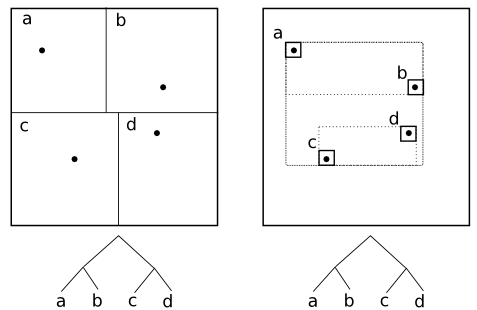
\includegraphics[width=10cm]{illustrations/kdTree_trackletTree.png}
\caption{Two possible ways of constructing a KD-Tree over four points.}
\label{trackletTree}
\end{figure}

The former type of tree is simpler to construct (and perhaps easier to
visualize when debugging).  This is the type of tree used in most the
other algorithms, which perform range searches and thus can extend
handle their error bars per-query by extending their ranges as needed.
However, the latter type of tree is the one needed for linkTracklets,
and is implemented by the KD-Tree subclass {\tt TrackletTree} in {\tt
  TrackletTree.cc}.


\paragraph{Performance Enhancements for Acceleration Range Calculation}
As noted earlier, the function {\tt updateAccBoundsReturnValidity},
which implements the equations \ref{maxAcc} and \ref{minAcc},
accounts for most of the CPU time spent in linkTracklets.  Thus,
optimizing performance in this section of code is critical.

Rather than evaluate all arguments to $\min$ and $\max$ functions at
the outset, the code attempts to evaluate each possible argument. If
it becomes clear at any point that inevitably $minAcc > maxAcc$, then
we know that the search can be pruned and the function returns
immediately.

As an additional optimization, we start with $minAcc$ and $maxAcc$ set
to the values used by our caller in the recursive searching. We know
that the caller was examining two endpoint nodes which were either
equal to or a parent of our current nodes, and thus our parents
$(minAcc, maxAcc)$ range will be greater than the one we
calculate. (For the initial start of the recursion, we use the
user-specified min/max acceleration thresholds, because we do not care
about any values outside this range anyway.)  By doing this, we
actually have a $maxAcc$ value available as soon as we calculate our
first possible $minAcc$ value and vice-versa; this allows the earliest
possible termination.  However, it does make the code somewhat more
confusing to read.

This confusion is somewhat amplified by the fact that this same {\tt
  updateAccBoundsReturnValidity} function is used for filtering
support nodes.  In this case, the initial $minAcc$ and $maxAcc$ values
are taken from the acceleration range calculated when examining the
endpoint nodes $nodeA$ and $nodeB$, since we are not interested in
finding acceleration values which connect $nodeA$ and a support node
unless they also connect the support node to $nodeB$.








%%%%%%%%%%%%%%%%%%%%%%%%%%%%%%%%%%%%%%%%%%%%%%%%%%%%%%%%%%%%%%%%%%%%%%%%
%%      TRACK FILTERING
%%%%%%%%%%%%%%%%%%%%%%%%%%%%%%%%%%%%%%%%%%%%%%%%%%%%%%%%%%%%%%%%%%%%%%%%
\subsection{Filtering of Tracks}
\subsubsection{Higher-Order Fits and Chi-Squared Probability Filtering}
\label{trackFilters}
Some more information on implementation of Tim's fitting and
chi-squared filter and the software. Stats on ground-truth fitting,
possible needs for improvements.

\subsubsection{Subset Removal}
\label{subsetRemoval}
Some tracks are {\bf subset tracks} of other tracks; that is,
occasionally detections linked by one track found by linkTracklets
will be a subset of those linked by another track in the same output
set.  This can arise for a variety of reasons, but occurs most
commonly when a real object generates tracklets on four or more nights
within a linking period. We generally expect that these subset tracks
are unhelpful, and because they increase the size of the set of tracks
sent to orbit determination, they are possibly costly.

Finding and removing subset tracks could be accomplished with a very
naive double-for loop over the set of tracks, but of course this does
not scale to larger data sets ($O(n^2)$ for $n$ tracks).  A more
efficient algorithm uses a detection-to-track ``reverse-map'' $R$,
which maps from each detection to the set of tracks holding that
detection.  This is easy to construct for a set of tracks $T$:

\begin{algorithmic}
  \FOR{$t_i \in T$}
  \STATE $R[d_j] = \{\}$
  \ENDFOR
  \FOR{$d_j \in t_i$}
  \STATE $R[d_j] = R[d_j] \cup t_i$
  \ENDFOR
\end{algorithmic}

We may then use the algorithm from
Figure~\ref{subsetRemovalAlgorithm}, which makes use of this
reverse-map.  The underlying idea is this: for each track $t_i$, we
seek to find any track containing all the detections in $t_i$; any
track containing all these detections must be equal to or a superset
of $t_i$.

\begin{figure}[h!]
\begin{algorithmic}
\FOR{$t_i \in T$}
  \STATE candidates = $T$
  \FOR{$d_j \in t_i$}
    \STATE candidates = candidates $\cap$ $R[d_j]$
  \ENDFOR
  \IF{$|$candidates$| >$ 1}
    \STATE $t_i$ is a subset of some other $t_j \in T$; discard it
  \ELSE 
    \STATE keep $t_i$
  \ENDIF
\ENDFOR
\end{algorithmic}
\caption{Psuedocode for the subset removal algorithm}

\label{subsetRemovalAlgorithm}
\end{figure}

Subset tracklets can also occur when collapseTracklets is used.  The
same algorithm and software can be used to remove subset tracklets
from a set of tracklets as well.

The reverse-map is implemented with a C++ {\tt std::map}, allowing
logarithmic-time lookups, and its contents are C++ {\tt std::set}s,
which allowing linear-time intersection calculations.  However, both
structures are implemented with trees; between the tracks themselves
and these tree structures, this algorithm can require significant
amounts of memory, and no distributed-memory equivalent is currently
known to us.  Fortunately, we have had good luck with distributed
shared-memory approaches for large data sets {\bf self-cite?}.



\subsection{Notes on Software Interfaces}

\subsubsection{Accomodations for Large Data Sets}
\label{largeData}
Over the course of our experiments, we discovered that under some
circumstances, tools may return some very large data sets - larger
than the memory available on our development machines.  Though RAM
sizes may grow over time, it is likely that DayMOPS users will
continue to experiment with increasingly dense noise or loose limits,
resulting in increasingly large numbers of tracklets or tracks.

To help deal with this problem, the {\tt  findTracklets} and
{\tt linkTracklets} functions can be configured to output their results
in various ways; they can be configured either to store their results
in memory and return them (much like a normal function call) or to
return nothing and write results directly to file.  If the user is
confident that the data set to be returned will fit in memory, the
former is more elegant, but for our experiments we always write to
file first, in case the number of tracklets or tracks discovered is
large.

The {\tt findTracklets} and {\tt linkTracklets} functions each take as
an argument an object of type {\tt findTrackletsConfig} or
{\tt linkTrackletsConfig}; each type has a public member variable
called {\tt outputMethod} which can be set.  {\tt findTracklets.h} and
{\tt linkTracklets.h} each contain enum types which can be used to set
these flags.

Dealing with larger-than-memory data sets as input to our software
tools is a more significant problem.  We generally assume that the
number of input detections will fit in memory, and that KD-Trees of
these detections will also fit in memory.  This has always been the
case, and fortunately it is easy to predict whether a set of
detections will fit in memory or not.  However, the number of
tracklets or tracks may, depending on the data and configuration of
the software, grow to be quite large, and is not trivially
predictable.  For software which uses tracklets or tracks as its input
data and operates on them in bulk (including {\tt collapseTracklets},
{\tt removeSubsets}, and {\tt linkTracklets}), this may be problematic;
see section \ref{parallelization} for more information on this
problem.









\section{Metrics \& Scaling of DayMOPS}

Current development efforts have focused on the sky-plane tracking
phase of DayMOPS, as all later processing is dependant on its
success. Existing orbit determination packages claim a high rate of
success for accurate Orbit Determination (OD) given a correctly-linked
track, and should correctly reject false tracks in nearly all cases
\citep{Milani2006}. As a result, we expect that the ability of the
system to successfully generate Moving Objects data products for solar
system objects given to DayMOPS will be determined primarily by the
sky-plane tracking component and its ability to send useful tracks to
OD.  We also expect the overall resource usage of the DayMOPS system
will be calculable given the runtime of the sky-plane tracking
component, the number of tracks it passes to OD, and the per-track OD
time of our OD package.  As a result, carefully studying the behavior
and output of the sky-plane linking should provide a reasonable
estimate of the resource usage of all of DayMOPS object discovery.

% NightMOPS RESOURCE USAGE?!

%% In this section, we will present metrics used to evaluate the
%% usefulness of the sky-plane tracking approach, the correctness of our
%% software implementation, and usefulness of filters. We also
%% investigate the expected resource usage of our software and expected cost
%% of performing OD on its output.

\subsection{Approximation models}

\textbf{TBD: Put Yusra's findings here, and Tim's}



\subsection{Linking Algorithms}



\subsubsection{Metrics for End-to-end Evaluation of Sky-plane Linking}
MOPS can generate a useful orbit, and thus a Moving Object, for an
object if it is observed sufficiently for OD to be performed (6
observations from at least 3 nights is the usual rule) and a track
containing those observations is correctly generated by DayMOPS and
passed to its OD phase.  An object for which such a track is generated
by DayMOPS is considered to be \textbf{found} by the DayMOPS pipeline.

Despite the best efforts of the telescope's cadence, not all objects
are observed in a manner such that they can generate an OD-worthy
track.  We refer to an object which is observed with a cadence
sufficient for an OD-worthy track as a \textbf{findable} object.  When
running simulations, determining whether or not a given object is
findable is fairly straightforward: by using \textit{a priori}
knowledge of when its simulated detections occurred, we can simply
measure the time intervals between these detections and determine
whether the time interval were sufficient for tracklet generation and
track generation.  Note that the sky-plane velocities/accelerations of
the objects are \textit{not} used in deciding whether an object is
considered findable.


To understand net cost and success of our linking, the number of
objects found and the cost of finding them is likely sufficient.
However, when measuring and optimizing the internal behavior of the
DayMOPS system, it is helpful to study the quality and quantity of the
intermediate data structures used. Thus, we present a few additional
metrics as well.

The total number of tracks or tracklets is of significant concern when
estimating the resource usage of the system.  The number of tracklets
will be a major factor in the predicting the workload of track
generation, and the number of tracks should entirely decide the size
of the workload for OD.  As such, we measure the \textbf{number of
  tracks} and \textbf{number of tracklets}.  

Correctly-linked tracks and tracklets are referred to as \textbf{true
  tracks} and \textbf{true tracklets}. We present the percentage of
tracklets and tracks which are true in our results. Note that it is
expected that multiple correctly-linked tracklets and/or tracks may be
generated for a given found object. As such, we expect the number of
true tracks and tracklets to significantly exceed the number of found
objects.  Nonetheless, we find that checking the true/false ratio of
tracklets and tracks helps to illustrate the quality of linkages used
as input to the track generation software and to OD.

%% \textbf{consider a paragraph on object coverage; we will need to
%%   update my existing code if we use it.}




\subsection{Experiments With A Simulated LSST Asteroid Detection Catalog}

To test MOPS, we generated one month of simulated asteroid detections,
based on the image cadence of the Operations Simulator (run 3.61)
between the dates 51029 and 51061, for one month of data.  Images from
around the full sky were used.  Simulated asteroid detections were
generated by applying ephemeris generation to a statistically viable
solar system model containing 11 million objects \citep{Grav2011}.
Objects which should have been visible based on their position,
magnitude, image filter, and seeing conditions for a given image were
recorded into a detection catalog.  Plausible per-image levels of
astrometric error were added to the detection locations.

\begin{figure}[ht!]
\centering
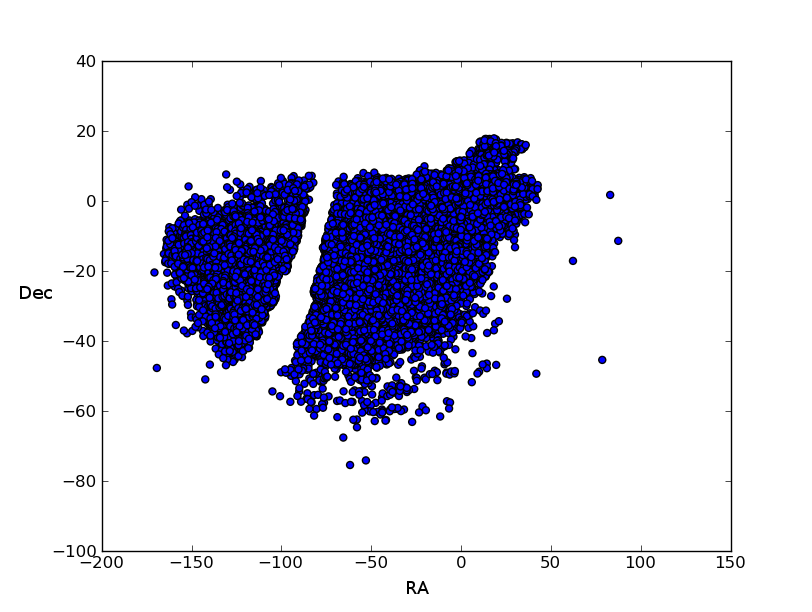
\includegraphics[scale=.7]{newIllustrations/fullSkyYear5_sourcesScatter.png}
\caption{A reduced-density plot of simulated asteroid detections
  (DiaSources) used in our simulated catalog.}
\label{diasPlot}
\end{figure}

A plot of some of the detections used in the simulation is presented
in figure \ref{diasPlot}.  As is visible in the plot, four of the
twenty-two fields had missing data due to a software error.  We expect
that the presence of this flaw in the data should not significantly
affect the conclusions reached from our experiments.









\subsubsection{Choosing the Linking Time-Window}

As expected in production, we attempted to generate tracklets between
any pair of images separated by more than 15 minutes and less than
90 minutes.  However, to speed up the track generation phase, we
attempted to link tracklets if they were separated by $\leq$ 15 days;
in production, it is expected that this number will be 30.  These
numbers should be consistently true across all experiments presented
here.


\subsubsection{Choosing Velocity and Acceleration Limits}
\label{velAccLimits}
\begin{figure}[ht!]
  \centering
  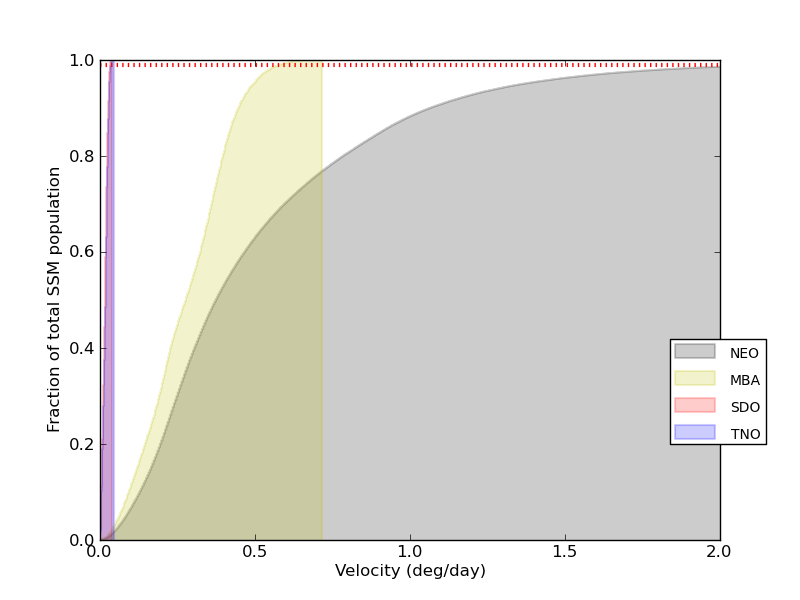
\includegraphics[width=13cm]{illustrations/mopsplots/aug2011/n_velocity.png}
  \caption{A cumulative histogram of solar solar system object
    sky-plane velocities, organized by classification.  Note that only
    the near-earth objects have higher velocities than main-belt
    asteroids.}
  \label{velSurvey}
\end{figure}

\begin{figure}[ht!]
  \centering
  \subfloat[Apparent Accelerations in Right Ascension over 15 Days]{
    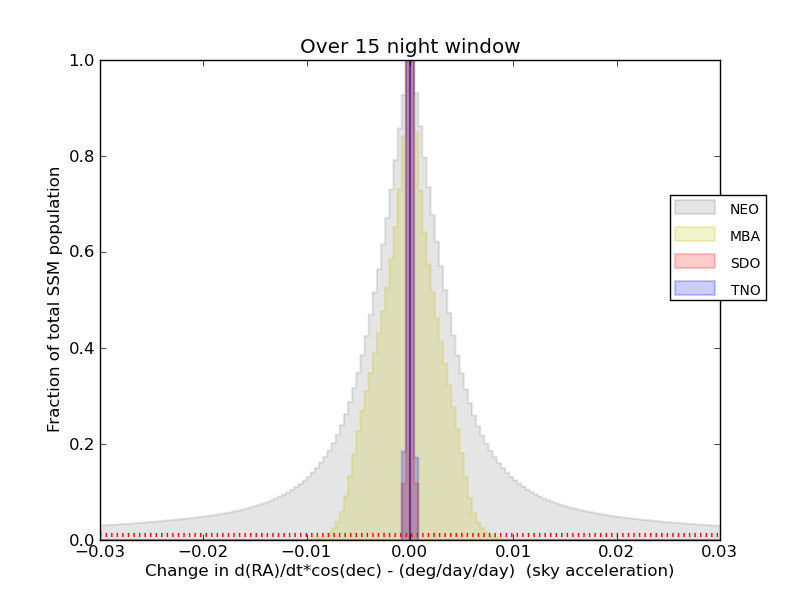
\includegraphics[width=8cm]{illustrations/mopsplots/aug2011/n_accel_ra_15.png}
    }
  \subfloat[Apparent Accelerations in Right Ascension over 30 Days]{
    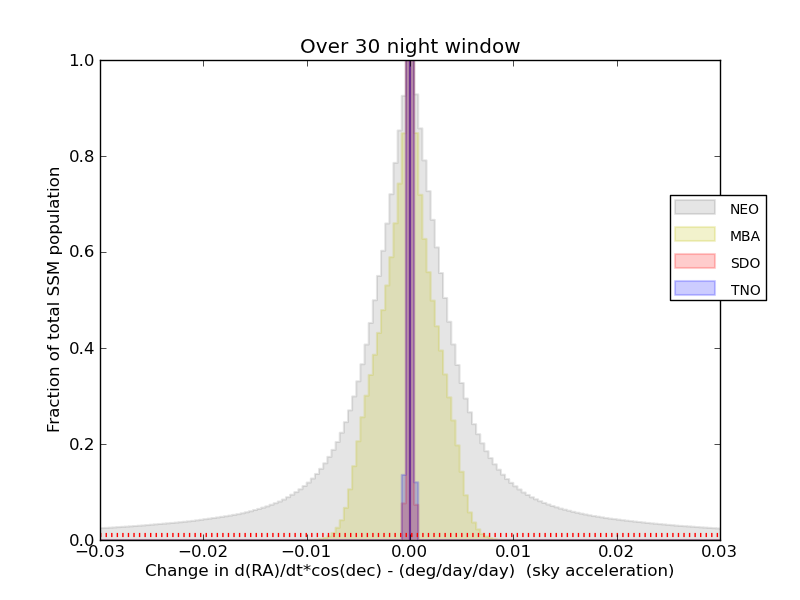
\includegraphics[width=8cm]{illustrations/mopsplots/aug2011/n_accel_ra_30.png}
    }

  \subfloat[Declination Apparent Accelerations in Declination over 15 Days]{
    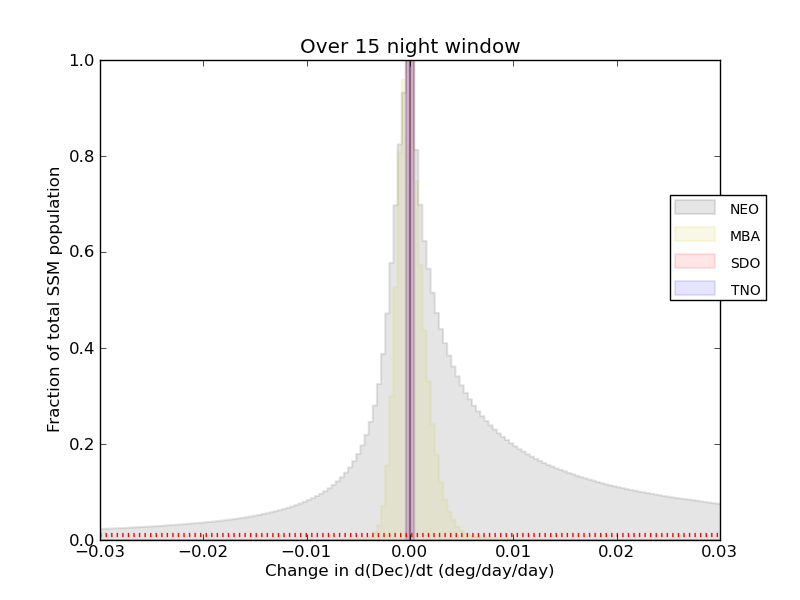
\includegraphics[width=8cm]{illustrations/mopsplots/aug2011/n_accel_dec_15.png}
    }
  \subfloat[Declination Apparent Accelerations in Declination over 30 Days]{
    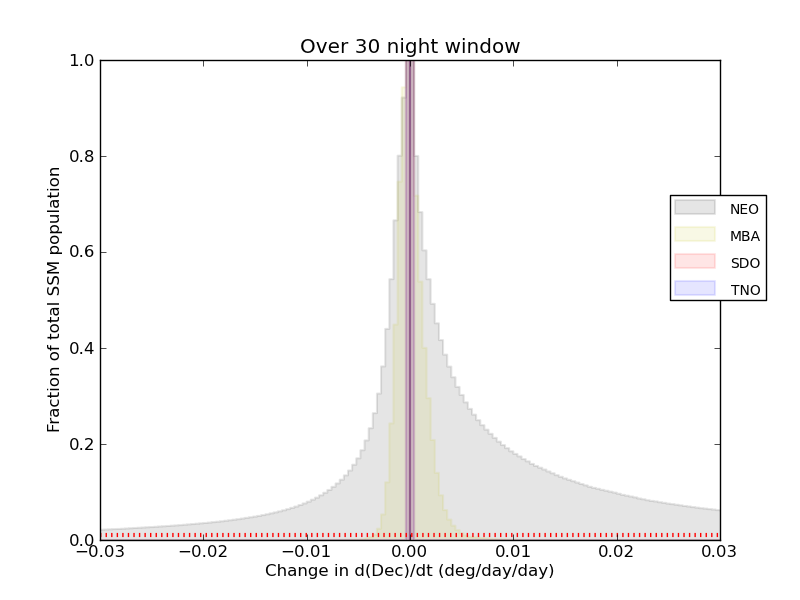
\includegraphics[width=8cm]{illustrations/mopsplots/aug2011/n_accel_dec_30.png}
    }
  \caption{Normalized histograms of sky-plane accelerations of several
    classes solar system objects in the RA and declination, with
    objects grouped by classification.  Histograms are presented for
    changes over 15 days and 30 days. The best-fit accelerations vary
    slightly given the size of the window; this is due to
    non-quadratic factors not included in the simple quadratic model.
    15 day tracking windows are used in the experiments presented in
    this document, but we expect to move to 30 day windows in the
    future.  In both cases, virtually all MBAs, and all other objects
    except NEOs, should have accelerations between -.02 and .02
    deg/day$^2$ in both axes.}
  \label{accSurvey}
\end{figure}


In order to determine reasonable limits on velocity and acceleration
of various classes of solar system objects, a survey of the solar
system model \citep{Grav2011} was conducted, see figures
\ref{velSurvey}, \ref{accSurvey} for histograms
presenting the results of these surveys.

We found that a velocity limit of .5 deg/day and an acceleration limit
.02 deg/day$^2$ would be generally sufficient.  By examining the
detections on an object-per-object basis, we calculated that among the
186,344 objects seen with proper cadence for OD, 186,209 of these
(more than 99.9\%) should generate useful tracks given these limits.

%% see mops64: /mnt/raid/jmyers/variousDensities/fullDensity/maxV.5_15days/trueTracks/*.log





\subsection{Results}

All simulations were conducted on the Gordon cluster at San Diego
Supercomputing Center.  Because of the large memory requirements for
running MOPS, the vSMP nodes were used for all stages of computation.
Except for the scaling tests, 16 threads were used for all the runs.


\begin{figure}[ht!]
\centering
\begin{tabular}{|r l|}
\hline
Number of asteroid detections: & 36,311,037 \\
Number of non-asteroid detections: & 0 \\
Average detections per night: & 1,134,719 \\
 & \\
Number of tracklets found: & 12,890,181 \\
Number of true tracklets: & 6,859,331 \\
Tracklets \% true: & 53.2\%\\
Tracklet generation time: & 4,791 sec (1.33 hours) \\
Tracklet generation memory use: & 13.7 GB  \\
 & \\
Number of tracks found: & 10,423,382 \\
Number of true tracks: & 5,779,424 \\
Track \% true: & 55.4\% \\
Track generation time: & 36,237 sec (10.1 hours) \\
Track generation memory use: & 16.2 GB \\
 & \\
Number of found objects: & 854,037 \\
Number of findable objects: & 1,128,643 \\
Found / findable: & 75.7\% \\
\hline
\end{tabular}

\caption{Results from the MOPS run without noise.  Velocity limit was .5 deg/day, acceleration limit was .02 deg/day$^2$ and the track chi squared probability limit was .9.  Note that not quite one fourth of objects which should generate plausible tracks are rejected.}
\label{oneMonth}
\end{figure}

\subsubsection{Survey Efficiency}
Figure~\ref{oneMonth} shows in-depth stats for a survey without noise.
As in all our runs, track generation is far more expensive than
tracklet generation in terms of CPU usage, but both require
substantial amounts of memory.  Also note that nearly one fourth of
the findable objects (those which should generate useful tracks) are
not found.  We expect that this is because of overly-aggressive
filtering in the chi squared probability filter.


\subsubsection{Nightly Variance in Runtime}

The cost of running MOPS depends on a variety of factors which are
largely dependent on telescope operations, such as revisit rates and
the locations of revisits.  Figure~\ref{nightlyVariance} shows some of
the 


\begin{figure}[ht!]
  \centering
  \subfloat{
    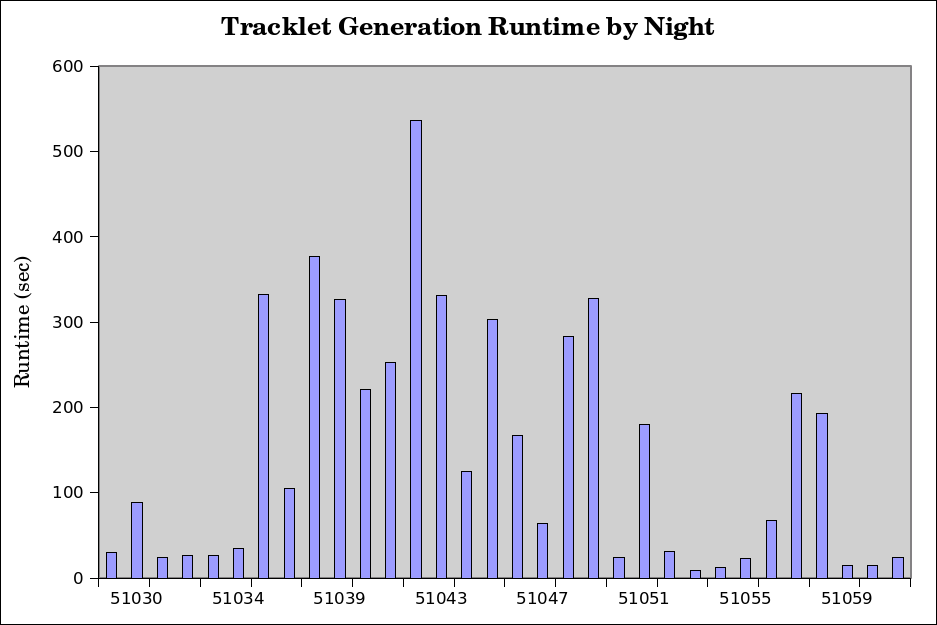
\includegraphics[width=12cm]{newIllustrations/tracklets_nightly.png}
    }
  \\
  \subfloat{
    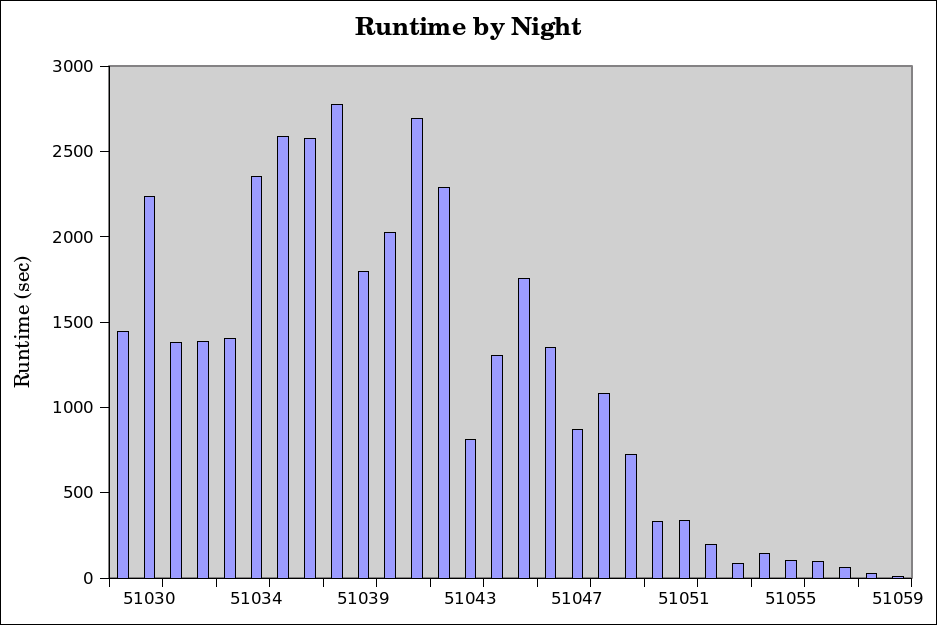
\includegraphics[width=12cm]{newIllustrations/tracks_nightly.png}
    }

  \caption{Per-night costs of tracklet generation and track
    generation. Also, in the track generation section,
    note that because only 31 sets of nightly tracklets were
    generated, later runs had less data in their window and thus ran
    considerably faster.  This is an artifact of the experiment and
    not a meaningful trend.}
  \label{nightlyVariance}
\end{figure}


\subsubsection{Scaling on Non-Asteroid Sources}

Actual images will contain DiaSources from non-asteroid sources:
variable stars, supernova, and image processing artifacts (e.g. from
bright stars) will also be present.  Because the quality of image
processing is not known, we added non-asteroid ``noise'' detections to
images at varying rates.  At each rate, a fixed $n$ noise detections
were added to each image, with locations chosen at random.  We
successfully ran MOPS using densities as high as 5,000 non-asteroid
sources per image.  After adding 10,000 non-asteroid sources per
image, tracklet generation was possible but linking tracklets into
tracks was too slow - at over 48 hours for a single night of
searching, it exceeded the wall-clock limit on Gordon jobs.

Figure~\ref{noiseScaling_detections} shows some information about the
detection catalogs generated at each of the noise densities.  For each
of these catalogs, tracklet generation was performed for each of the
31 simulated nights of observation; results can be seen in
Figure~\ref{noiseScaling_tracklets}.  As expected, increasing numbers
of false detections lead to worse-than-linear increases in mislinkage.
This lead to worse-than-linear increases in computational costs for generating the
tracklets, both in terms of CPU and memory usage.

The tracklets generated in the tracklet generation test were used to
test scaling of track generation.  For reasons of time, we only
attempted to search for tracks starting on the first night of
observation.  Results are presented in
Figure~\ref{noiseScaling_tracks} and Figure~\ref{noiseScaling_found}.
The track generation scaled well on the additional tracklets (which
were primarily due to mislinkage).  We saw only modest increases in
the number of output tracks and runtime for linkTracklets.  Also note
that the number of objects found remained nearly constant across the
various runs.  



\begin{figure}[ht!]
\centering

\begin{tabular}{|c c c c|}
\hline
Per-Image Noise Density & Total number of detections & \% noise detections &  \\ 
0             & 36,311,037             & 0\%                          & \\
1,250         & 72,258,537             & 49.7\%          & \\
2,500         & 108,206,037            & 66.4\%          & \\ 
5,000         & 180,101,037            & 79.8\%          & \\
\hline
\end{tabular}
\caption{An overview of the detection sets used for the scaling tests on noise density.}
\label{noiseScaling_detections}
\end{figure}

\begin{figure}[ht!]
\centering

\subfloat[Number of tracklets generated at various noise density levels]
{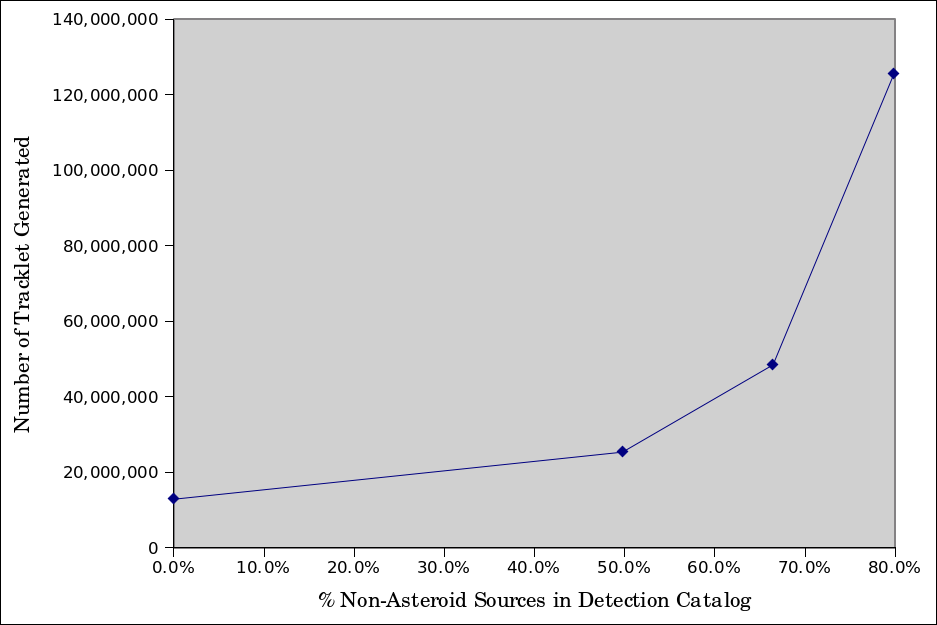
\includegraphics[width=8cm]{newIllustrations/tracklet_num.png}}
\subfloat[Tracklet \% true at various noise density levels]
{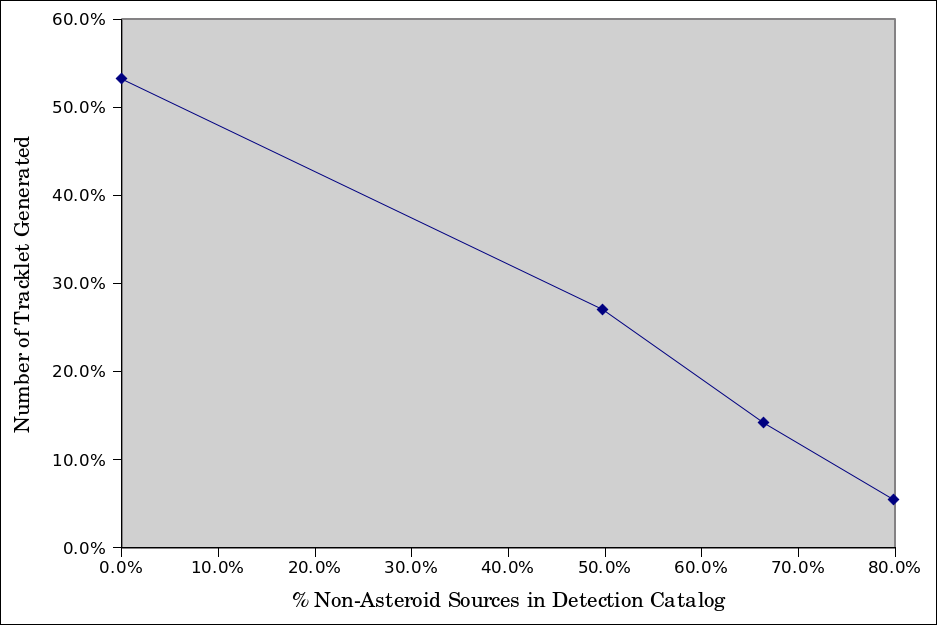
\includegraphics[width=8cm]{newIllustrations/tracklet_true.png}}
\\
\subfloat[Tracklet generation runtimes at various noise density levels]
{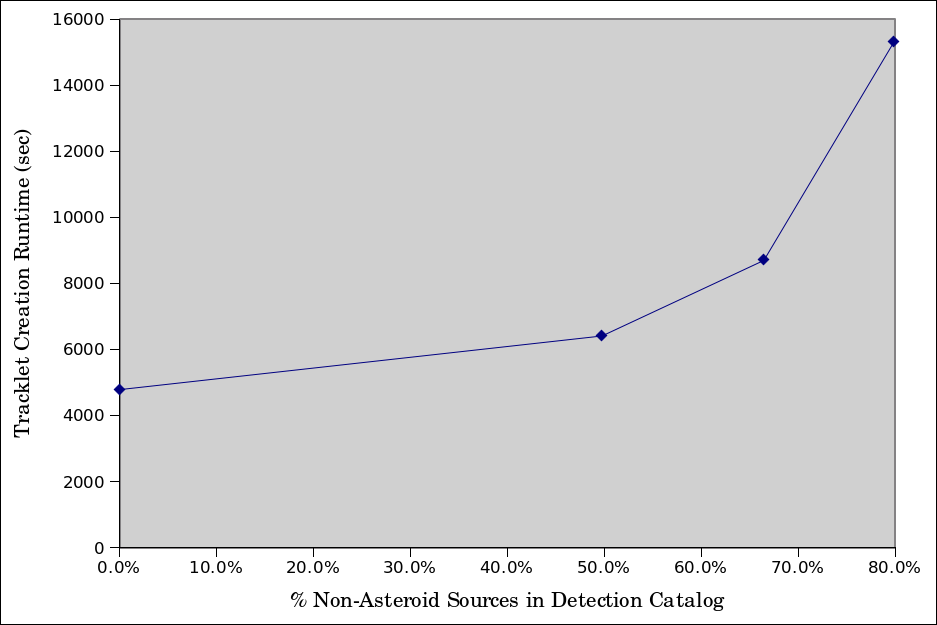
\includegraphics[width=8cm]{newIllustrations/tracklet_runtime.png}}
\subfloat[Tracklet generation memory use at various noise density levels]
{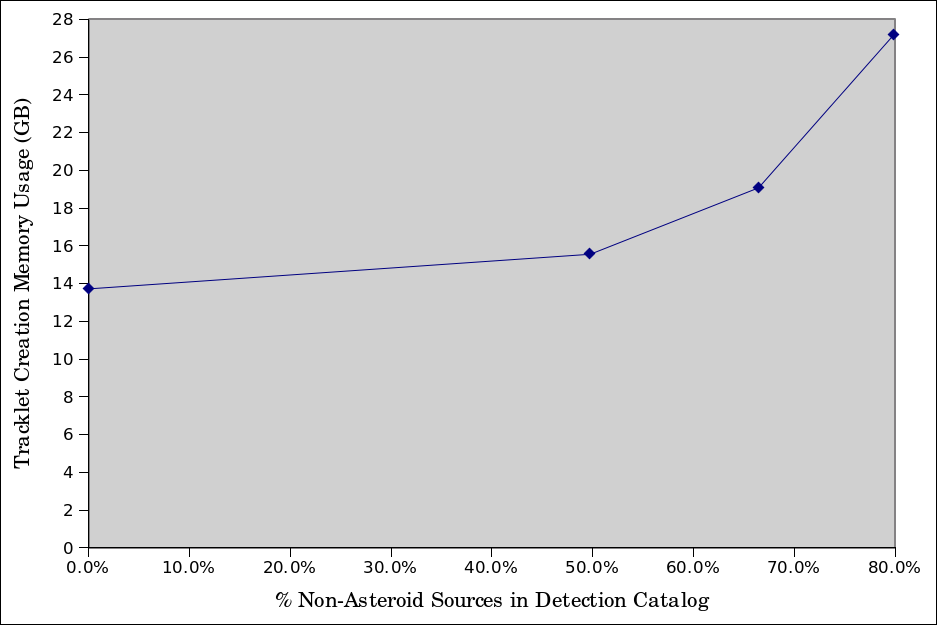
\includegraphics[width=8cm]{newIllustrations/tracklet_mem.png}}

\caption{Tracklets generated at varying densities of non-asteroid
  ``noise'' sources, and corresponding compute costs.  Each data point
  represents 31 days of tracklet generation.  The same asteroid
  catalog was used for each simulation, but increasing numbers of
  ``noise'' sources were added in each simulation (see
  Figure~\ref{noiseScaling_detections}). Note that the number of
  tracklets generated, and the computational costs to find them,
  increase quickly as noise density increases. This is apparently due
  to the increase of mislinked ``false tracklets''. }
\label{noiseScaling_tracklets}
\end{figure}


\begin{figure}[ht!]
\centering

\subfloat[Number of tracks generated at various noise density levels]
{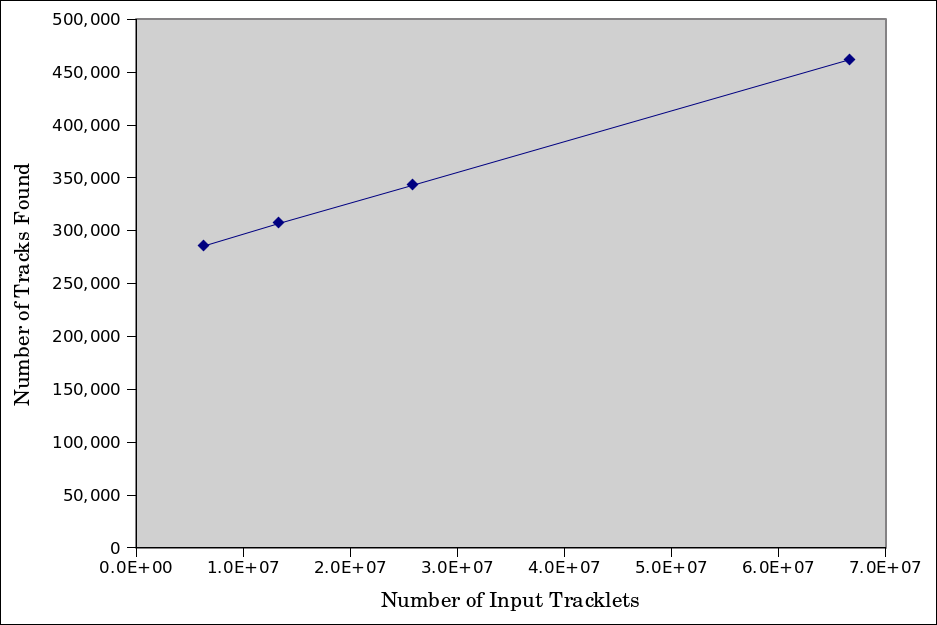
\includegraphics[width=8cm]{newIllustrations/track_num.png}}
\subfloat[Track \% true at various noise density levels]
{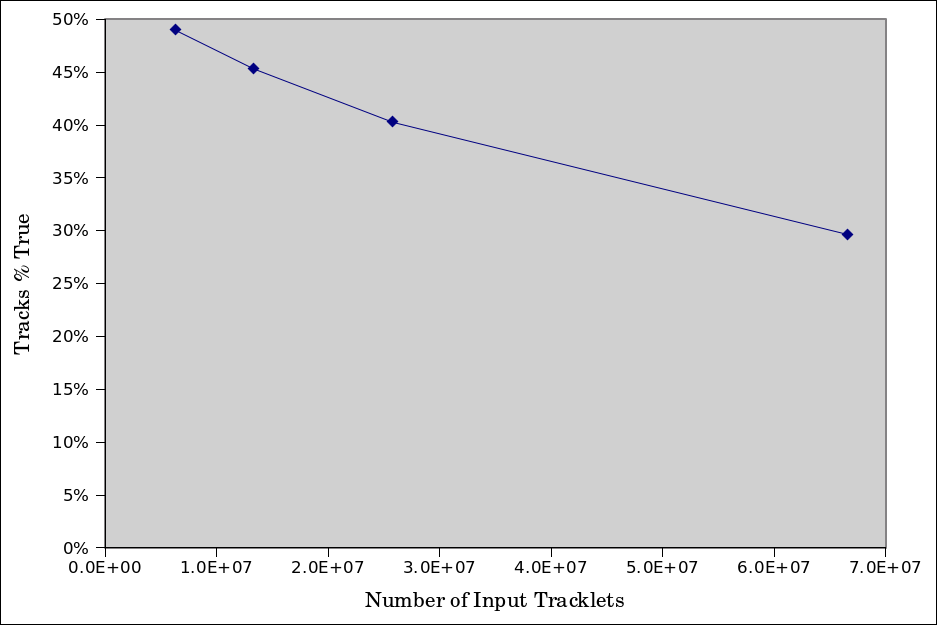
\includegraphics[width=8cm]{newIllustrations/track_true.png}}
\\
\subfloat[Track generation runtimes at various noise density levels]
{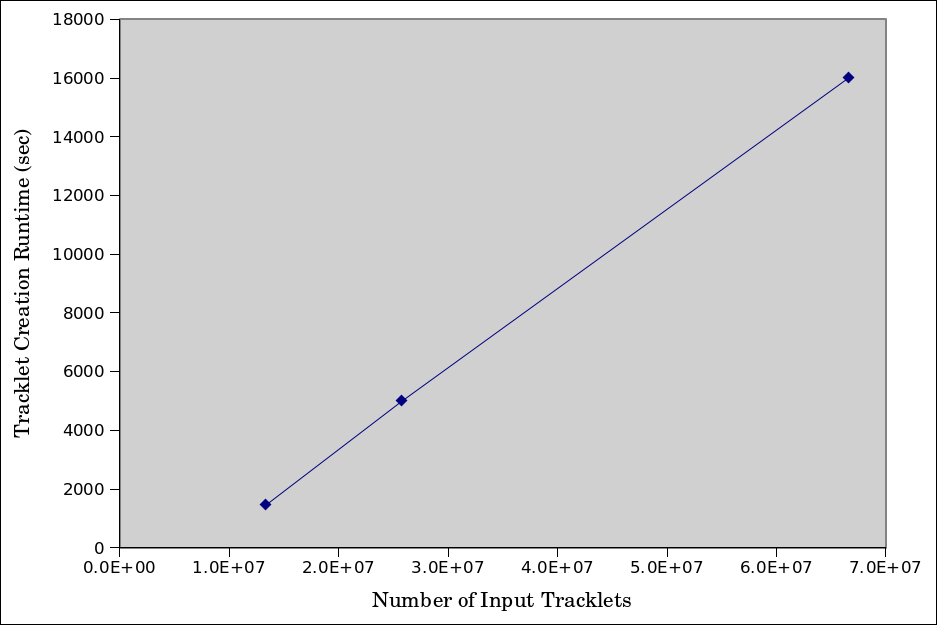
\includegraphics[width=8cm]{newIllustrations/track_runtime.png}}
\subfloat[Track generation memory use at various noise density levels]
{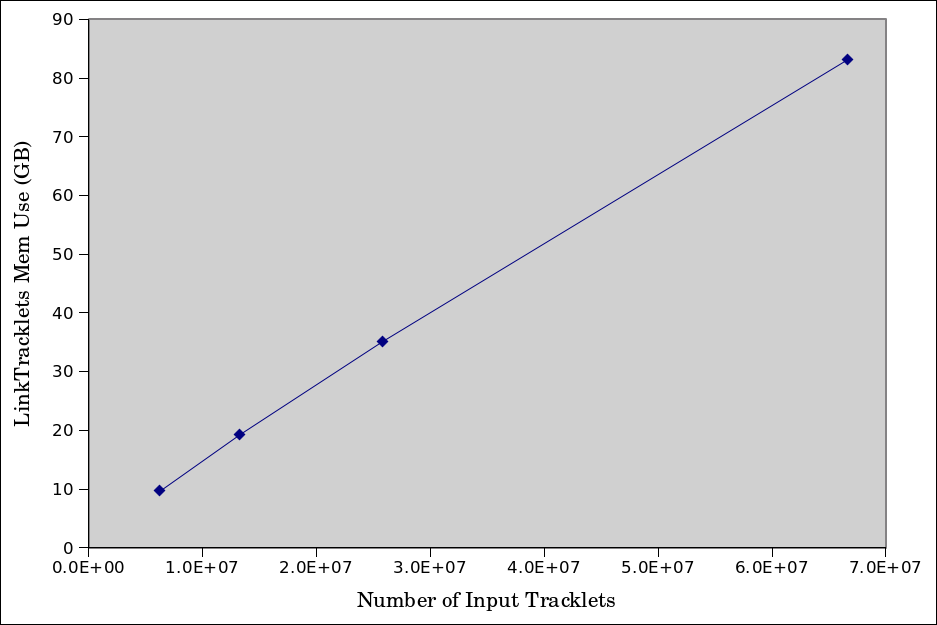
\includegraphics[width=8cm]{newIllustrations/track_mem.png}}

\caption{Tracks generated at varying densities of non-asteroid
  ``noise'' sources, and corresponding compute costs.  Detections
  catalogs with increasing numbers of noise detections
  (Figure~\ref{noiseScaling_detections}) and tracklets generated from
  these catalogs (~\ref{noiseScaling_tracklets}) were used to generate
  linkTracklets input. For reasons of time, each linkTracklets run
  attempted to find only tracks which started on the first night of
  data and ended anywhere within the first 15 days.}
\label{noiseScaling_tracks}
\end{figure}


\begin{figure}[ht!]
\centering
\begin{tabular}{|c c c|}
\hline

Noise Density & Number of Tracklets & Found Objects \\
0 & 6,312,807 & 55,982 \\
1,250 & 13,318,186 & 55,870  \\
2,500 & 25,824,121 &  55,751  \\
5,000 & 66,635,397 &  55,464  \\
\hline
\end{tabular}

\caption{Objects found by linkTracklets with varying densities of
  noise in the input catalogs.  Note that the number of objects found
  is only slightly affected by the presence of noise in the input
  catalogs.}
\label{noiseScaling_found}
\end{figure}



\subsubsection{LinkTracklets Scaling on Number of Threads}

\begin{figure}[ht!]
\centering
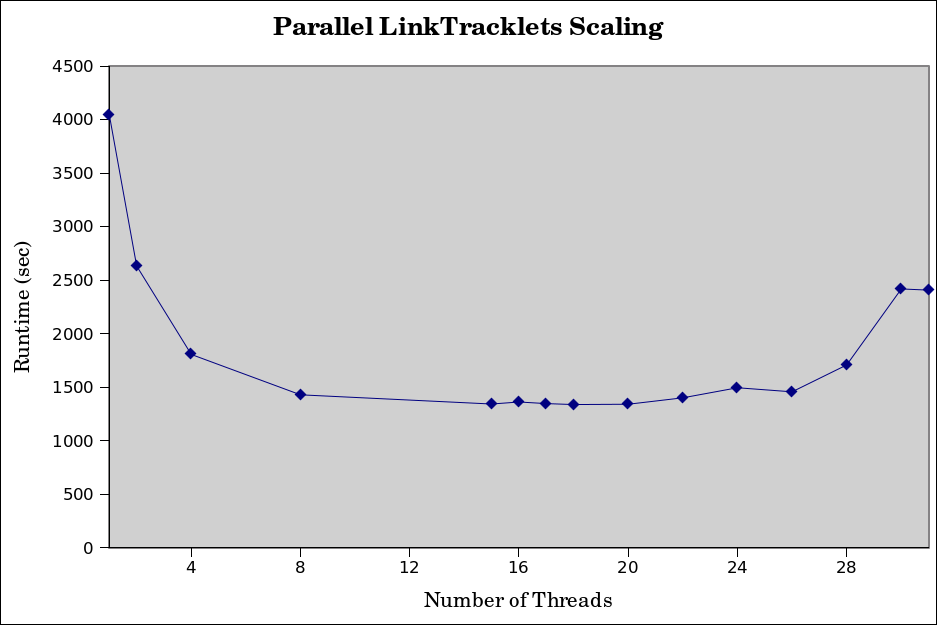
\includegraphics[width=16cm]{newIllustrations/linkTracklets_scaling.png}
\caption{LinkTracklets runtimes with varying numbers of threads.}
\label{threadScaling}
\end{figure}



\section{Implications for Survey Performance}
% tbd: expand this into its own file...
Talk here about OpSim, cadence, software limitations and science requirements.

\section{Risk Reduction}

Though the core algorithms of MOPS have been implemented in
LSST-appropriate style, further research and development are needed.



\subsection{Long Duration Survey Performance}

Current simulations cover fairly short time periods, and therefore
emphasize the problem of initial object discovery.  In the course of
the full survey, we expect that many detected sources will be
attributed to already-discovered objects.  Because initial object
discovery phases are relatively expensive and ephemeris calculation is
relatively fast, we expect that the resource usage of the system will
decline over time, as more objects are discovered and the size of
input catalogs is reduced.  This expectation needs to be verified and
quantified.

Attribution, precovery and Moving Object management and refinement of the
Moving Object table are not yet implemented in LSST-compliant software.
Developing this software should be a significant development task.
However, we hope that by using the algorithms from the PanSTARRS MOPS
we can avoid any significant research tasks.

To test this software, we will need to generate simulated input
catalogs which span longer time periods.  Accomplishing this will
require either significant compute-resources or improved tools for
generating input catalogs.


\subsection{Future Software Development Tasks}

\subsubsection{Filtering on Trailing for Near-Earth-Object Searching}

\label{neosTrailing}

Near-Earth Objects tend to have the highest sky-plane velocity.  This
presents a significant challenge; as we increase the maximum velocity
limit of our tracklet generation, the potential for mislinkage
increases significantly, leading to higher numbers of tracklets and
increased costs.  

Fortunately, fast-moving NEOs will generate visible trails in our
images.  By requiring all tracklets to show trails consistent with
their apparent sky-plane velocity, we expect that it will be possible
to filter most false tracklet linkages, thus rendering the problem of
NEO searching manageable.

The ability to filter on trailing is dependent almost entirely on our
ability to correctly identify trails in images.  Currently, the
ability of image processing to detect trails is not well quantified.  To
remedy this, we will need to generate simulated images which include
asteroid trails and send them to image processing; further refinement
of image processing algorithms may be neccesary.



\subsubsection{Distribution/Parallelization of Software}
\label{parallelization}

To meet the needs of full operations, DayMOPS will almost certainly
need to utilize some form of parallelism in order to reduce runtime.
For some components, such as orbit determination, this should be
easily achieved; others will require closer attention to detail.  We
have planned parallel or distributed versions for most components,
which are described below.  In some cases we have also experimented
with various initial implementations, which are noted.

%% do we need this?
%% \subsubsubsection{Tools And Methods}
%% \paragraph{Multithreading and OpenMP}
%% \paragraph{Distributed Shared Memory}
%% \paragraph{Full Distribution and MPI}


\subsubsubsection{Orbit Determination} Orbit Determination is
performed per-track; we expect that it will be slow only because the
number of tracks will be very large.  Thus, we expect that Orbit
Determination should be trivially parallel; simply divide the tracks
between various machines or CPU cores. 

\subsubsubsection{Parallel FindTracklets} The findTracklets section of
our pipeline tends to run very quickly.  For this reason, we do not
anticipate that parallelizing findTracklets will be necessary at all.
However, if we choose to parallelize it, then it should be trivial to
distribute the workload; one query is performed per input detection,
and each query is naturally independent, so it should be trivial to
parallelize the work at this level.  This could be accomplished by
changing the outer ``for'' loop to a ``parallel for'' loop, e.g. using
OpenMP.  We anticipate that the detections as well as the trees over
detections should fit in memory, making explicit distribution
unnecessary.

\subsubsubsection{Parallel CollapseTracklets} It has been our
experience that the collapseTracklets phase is generally quite fast,
and will likely not need parallelization.  One tree query will be
performed per tracklet, which provides a natural axis of parallelism.
However, there is potential for some contention between CPUs as we
normally check whether an input tracklet has been collapsed already by
a prior query, and if so, do not attempt to work with it.  Dealing
with this conditional will require synchronization between CPUs, which
could hamper performance.  It might also be ignored, perhaps allowing
the redundant work to happen in order to avoid the synchronization
costs.

\subsubsubsection{Parallel LinkTracklets} We have experimented with a
parallel, shared-memory linkTracklets implementation based on OpenMP.
The linkTracklets phase creates a tree of tracklets at each image
which generated tracklets, and attempts searching using each
temporally well-separated pair of trees as endpoint trees, with
intermediate-time trees as sources of possible support.  Each of these
searches is independent, so this provides a fairly natural axis of
parallelism.  However, this does not address the potential case where
the trees become larger than memory, which we have determined to be a
plausible problem.  To deal with this, we have used the kernel-level
distributed shared-memory provided by vSMP on the Dash and Gordon
clusters.  This way, a series of distributed machines provide the
appearance of a shared-memory system for OpenMP.  It may also be
possible to accomplish a similar effect by explicitly rewriting
linkTracklets to use a user-level distributed shared memory library
and MPI.  

\subsubsubsection{Distributed LinkTracklets} In case the implicit
memory sharing is not sufficient, it may be necessary to write an
explicitly distributed linkTracklets.  This was attempted by a CS
Master's student, Matt Cleveland, working with Prof. Dave Lowenthal.
The design was well-thought out but complex, leading to slow
implementation.  The distributed version was forked off before a
variety of changes to the serial version were made, and never merged
back.

The distributed linkTracklets held only the higher levels of trees and
the tracklets of the endpoint trees on the master node.  The master
node would attempt the linking algorithm on the higher levels of the
tree until it reached a terminal point; it would then attempt to
predict the amount of work needed to complete the linking and save the
state of the searching and estimated cost to a buffer.  Periodically,
the work items in the buffer are distributed to worker nodes, with
attention given to load distribution as well as cache issues,
attempting to minimize the amount of data which must be transferred to
worker nodes.


\subsubsubsection{Parallel Subset Removal}


\appendix
\section{About the KD-Tree Library}

\section{Helpful Metrics and Software Tools}
\subsection{Studying OpSim}
\subsection{Studying Tracks}



\bibliographystyle{apj}
\bibliography{baseline}




\end{document}
